\chapter{免疫球蛋白}
\begin{framed}
\noindent\textbf{【知识体系】}
\begin{center}
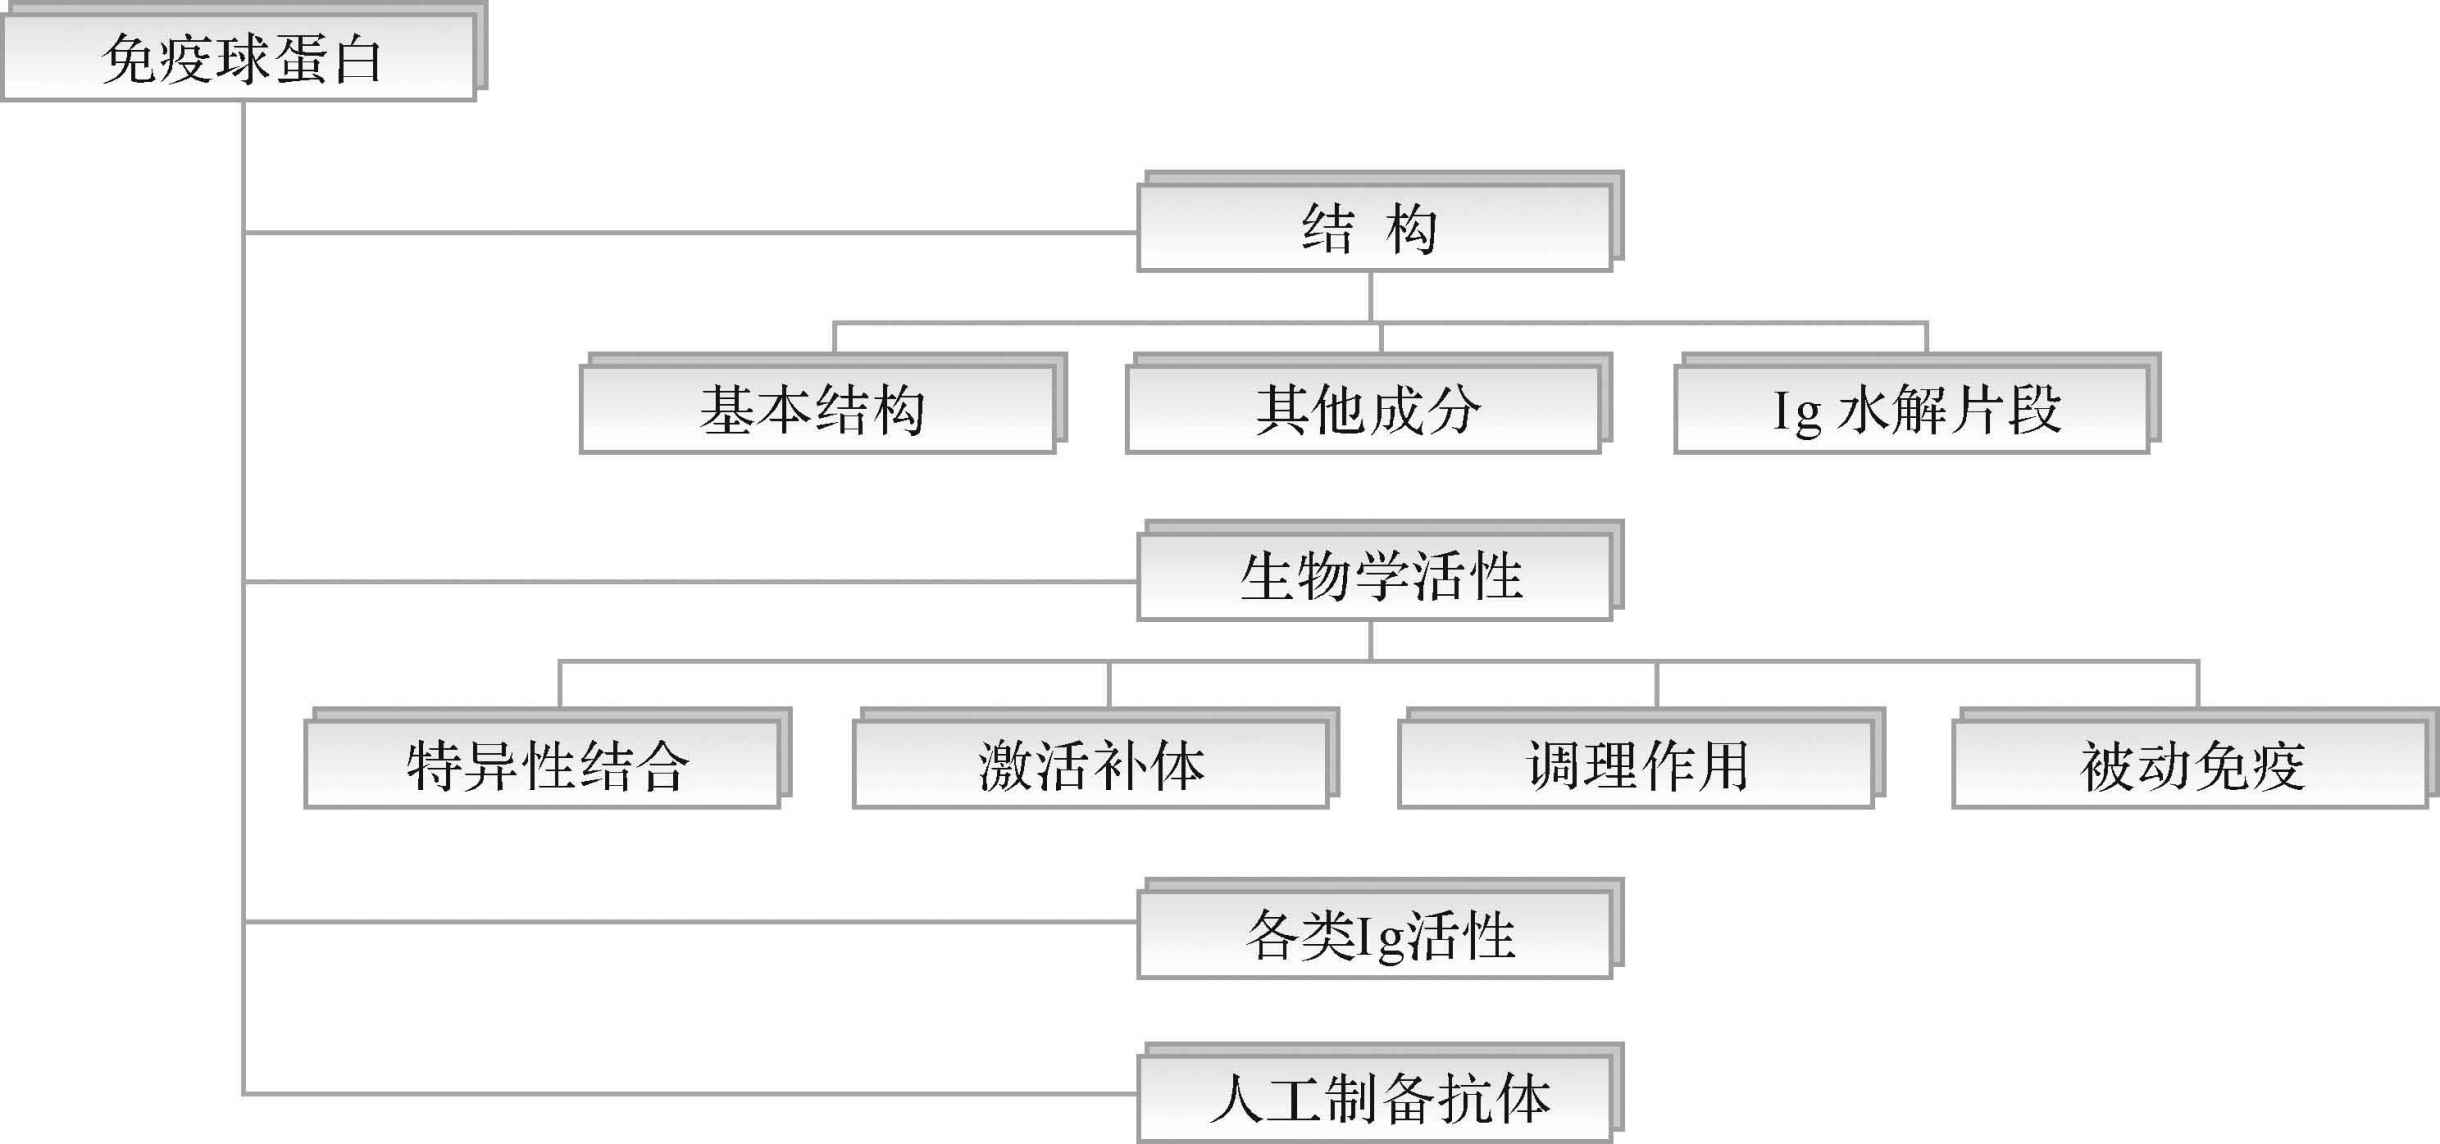
\includegraphics{./images/Image00060.jpg}
\end{center}
\noindent\textbf{【课前思考】}

机体注射疫苗后,体内的哪些成分增加?老弱病人要补充什么药物来增强其抵抗力?这是一种什么成分?是怎么产生的?有什么结构?有多少种类?在机体中起到什么样的作用?人工如何制备?医学上有何应用?

\noindent\textbf{【本章重点】}

1.免疫球蛋白的概念、结构、功能、种类;

2.五类免疫球蛋白的生物学活性;

3.单克隆抗体的概念、特点和医学意义。

\noindent\textbf{【教学目标】}

1.掌握免疫球蛋白的概念、结构、功能、种类;

2.掌握各类免疫球蛋白的生物学活性;

3.熟悉单克隆抗体的特点和医学意义。
\end{framed}

抗体(antibody,Ab)是介导体液免疫的重要效应分子,是B细胞接受抗原刺激后增殖、分化为浆细胞所产生的糖蛋白。早在19世纪后期,从Behring及Kitasato对白喉和破伤风抗毒素(antitoxin)的研究开始,人们陆续发现一大类可与病原体结合并引起凝集、沉淀或中和反应的体液因子,将它们命名为抗体。1939年,Tiselius和Kabat在对血清蛋白自由电泳时,根据它们不同的迁移率,将其分为白蛋白及α、β、γ球蛋白4个主要部分,并发现抗体活性存在于从α到γ的这一广泛区域,但主要存在于γ区,故曾片面地认为抗体即是γ球蛋白。1968年和1972年,世界卫生组织和国际免疫学会联合会的专门委员会先后决定,将具有抗体活性或化学结构与抗体相似的球蛋白统称为免疫球蛋白(immunoglobulin,Ig)。近年研究证实,免疫球蛋白和抗体在结构及功能上完全一致,因此可认为二者的概念等同。免疫球蛋白可分为分泌型(secreted
Ig,SIg)和膜型(membrane
Ig,mIg),前者主要存在于血液及组织液中,发挥各种免疫功能;后者构成B细胞表面的抗原受体,图\ref{fig4-1}为正常人血清电泳分离图。

\begin{figure}[!htbp]
 \centering
 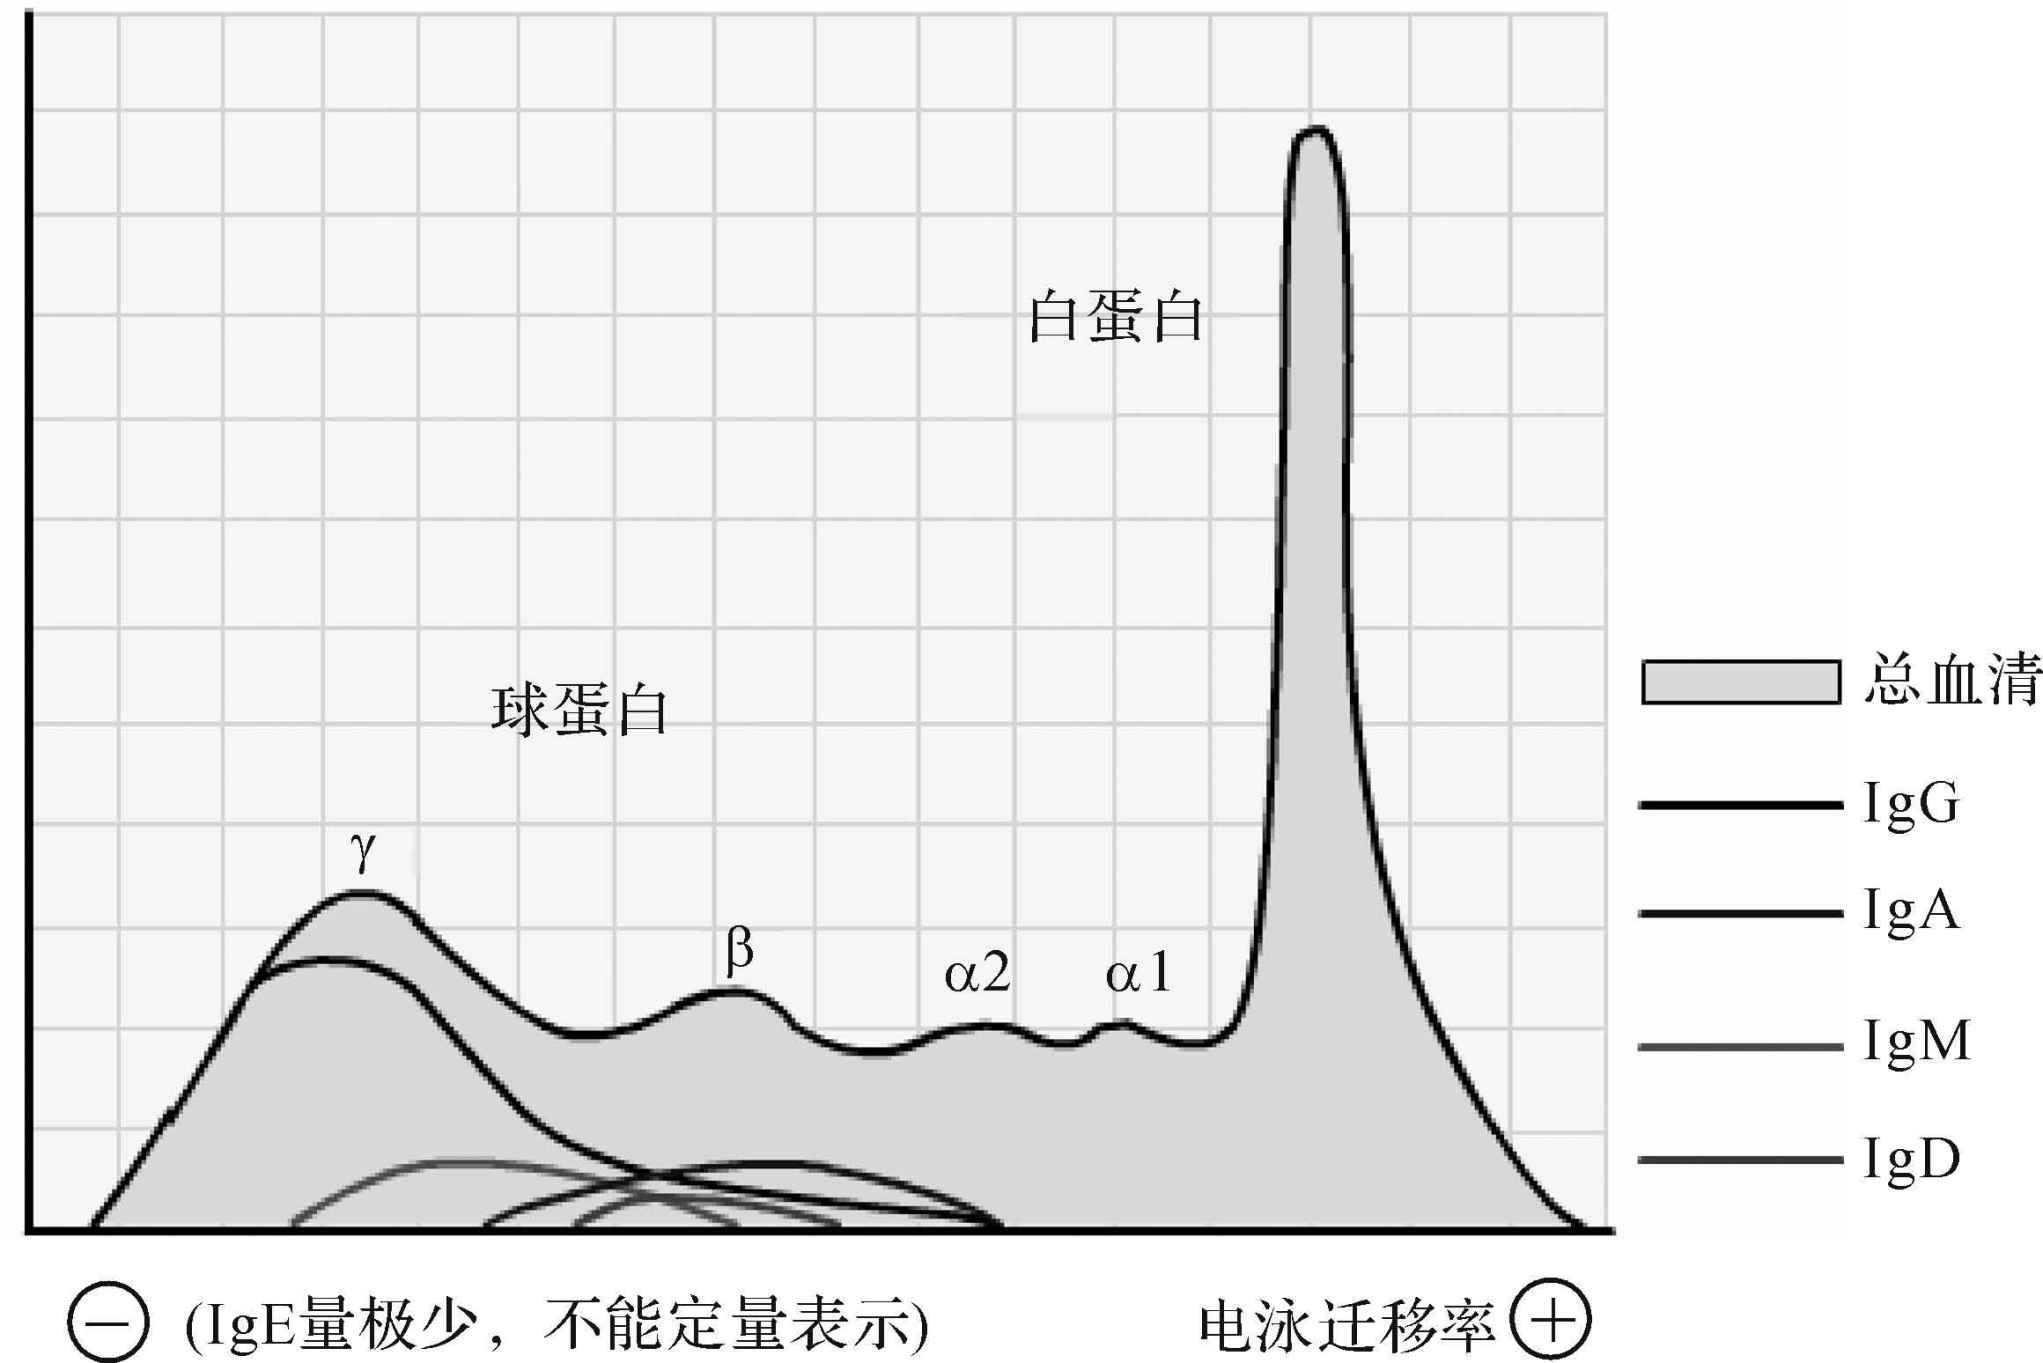
\includegraphics{./images/Image00061.jpg}
 \captionsetup{justification=centering}
 \caption{正常人血清电泳分离图}
 \label{fig4-1}
  \end{figure} 

\section{免疫球蛋白的结构}


\subsection{基本结构}

\begin{figure}[!htbp]
 \centering
 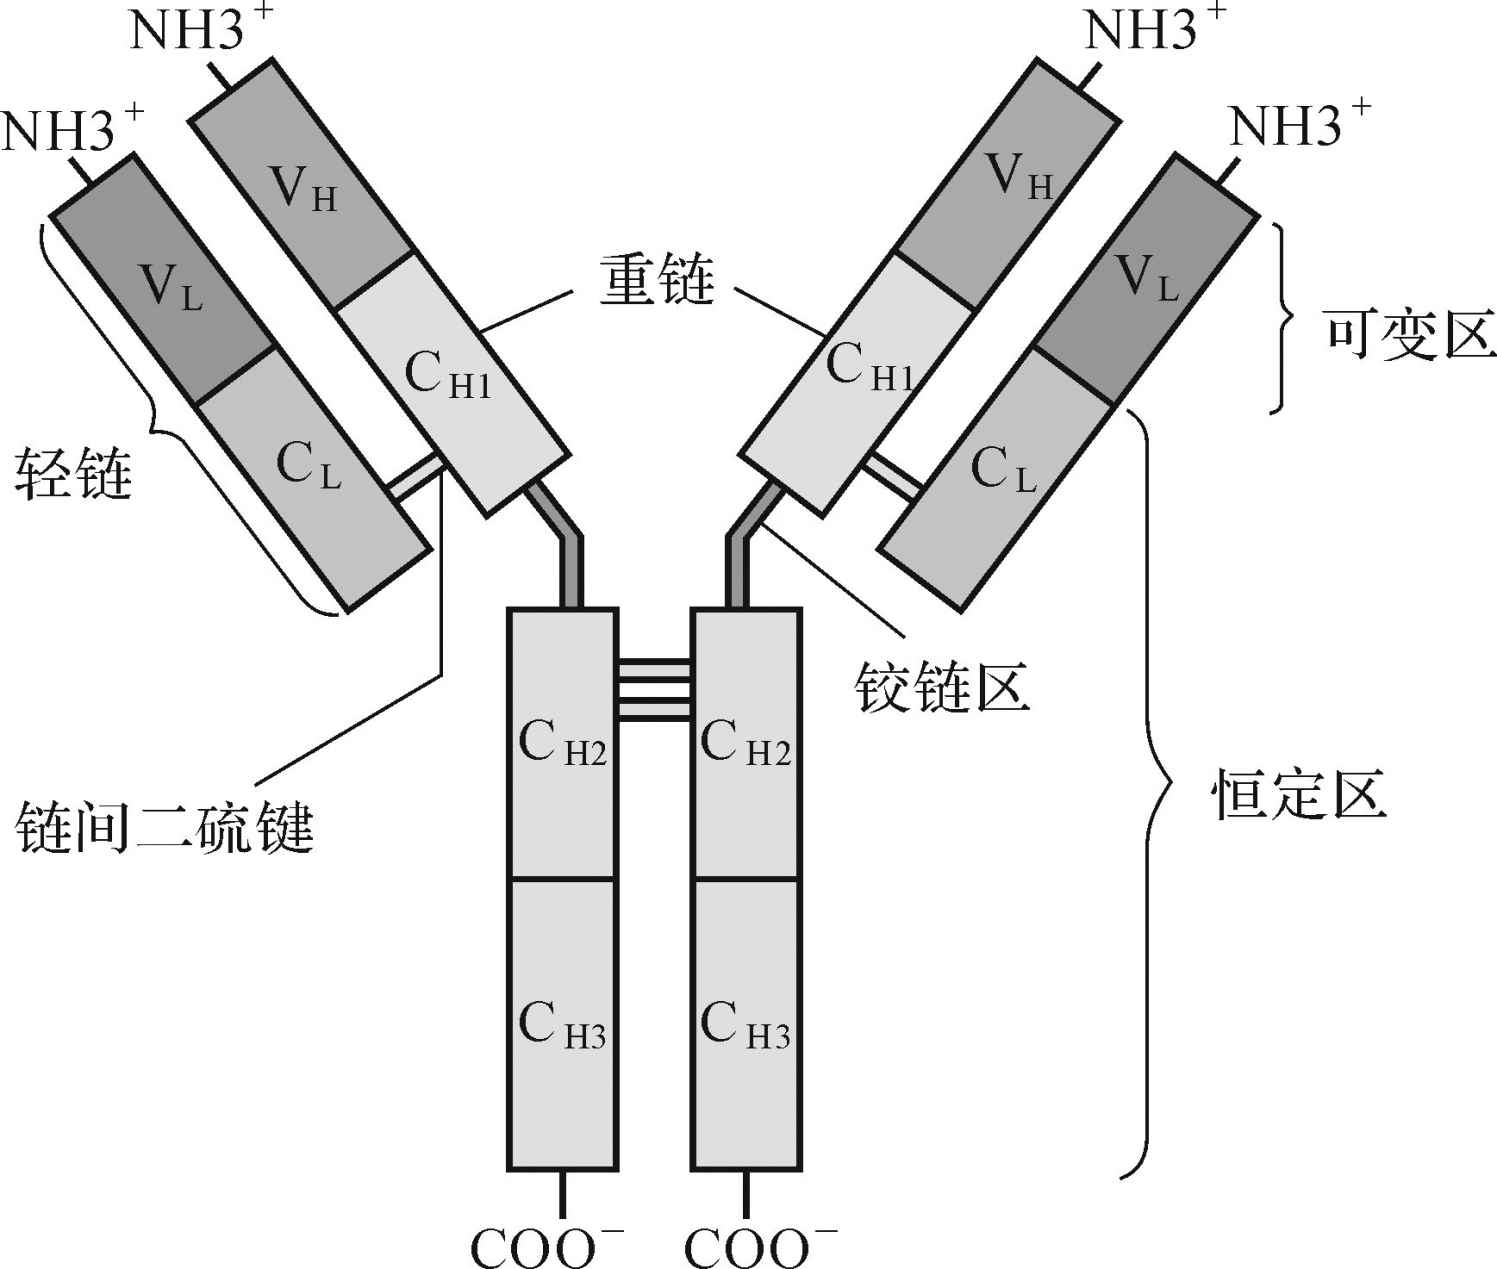
\includegraphics{./images/Image00062.jpg}
 \captionsetup{justification=centering}
 \caption{免疫球蛋白结构示意图}
 \label{fig4-2}
  \end{figure} 

免疫球蛋白分子的基本结构是一“Y”字形的四肽链结构,由两条完全相同的重链(heavy
chain,H)和两条完全相同的轻链(light
chain,L)以二硫键连接而成,如图\ref{fig4-2}所示。

(一)重链和轻链

免疫球蛋白重链由450~550个氨基酸残基组成,分子量约50~75
kD。重链可分为μ、δ、γ、α和ε链,据此可将免疫球蛋白分为5类(class)或5个同种型(isotype),即IgM、IgD、IgG、IgA和IgE。每类Ig根据其绞链区氨基酸残基的组成和二硫键数目、位置的不同,又可分为不同亚类(subclass)。

免疫球蛋白轻链含约210个氨基酸残基,分子量约25
kD。轻链分为κ和λ链两种,据此可将Ig分为κ和λ两型
(type)。一个天然Ig分子两条轻链的型别总是相同的,但同一个体内可存在分别带有κ或λ链的抗体分子。正常人血清中κ型和λ型免疫球蛋白浓度之比约为2∶1。根据l链恒定区个别氨基酸残基的差异,又可将λ分为λ1、λ2、λ3和λ4四个亚型。

(二)可变区和恒定区

比较不同Ig重链和轻链的氨基酸序列时发现,重链和轻链近N端约110个氨基酸序列的变化很大,其他部分氨基酸序列则相对恒定。免疫球蛋白轻链和重链中氨基酸序列变化较大的区域称为可变区(variable
region,V),分别占重链和轻链的1/4和1/2。免疫球蛋白轻链和重链中氨基酸序列较保守的区域称为恒定区(constant
region,C),其位于肽段的羧基端,分别占重链和轻链的3/4和1/2。重链和轻链V区(分别称为V\textsubscript{H}
和V\textsubscript{L}
)各有3个区域的氨基酸组成和排列顺序高度可变,称为高变区(hypervariable
region,HVR)或互补决定区(complementarity determining
region,CDR),分别为CDR1、CDR2和CDR3(图\ref{fig4-3})。CDR以外区域的氨基酸组成和排列顺序相对不易变化,称为骨架区(framework
region,FR)。V\textsubscript{H} 和V\textsubscript{L}
各有FR1、FR2、FR3和FR4四个骨架区。V\textsubscript{H}
和V\textsubscript{L}
的3个CDR共同组成Ig的抗原结合部位,负责识别及结合抗原,从而发挥免疫效应。

\begin{figure}[!htbp]
 \centering
 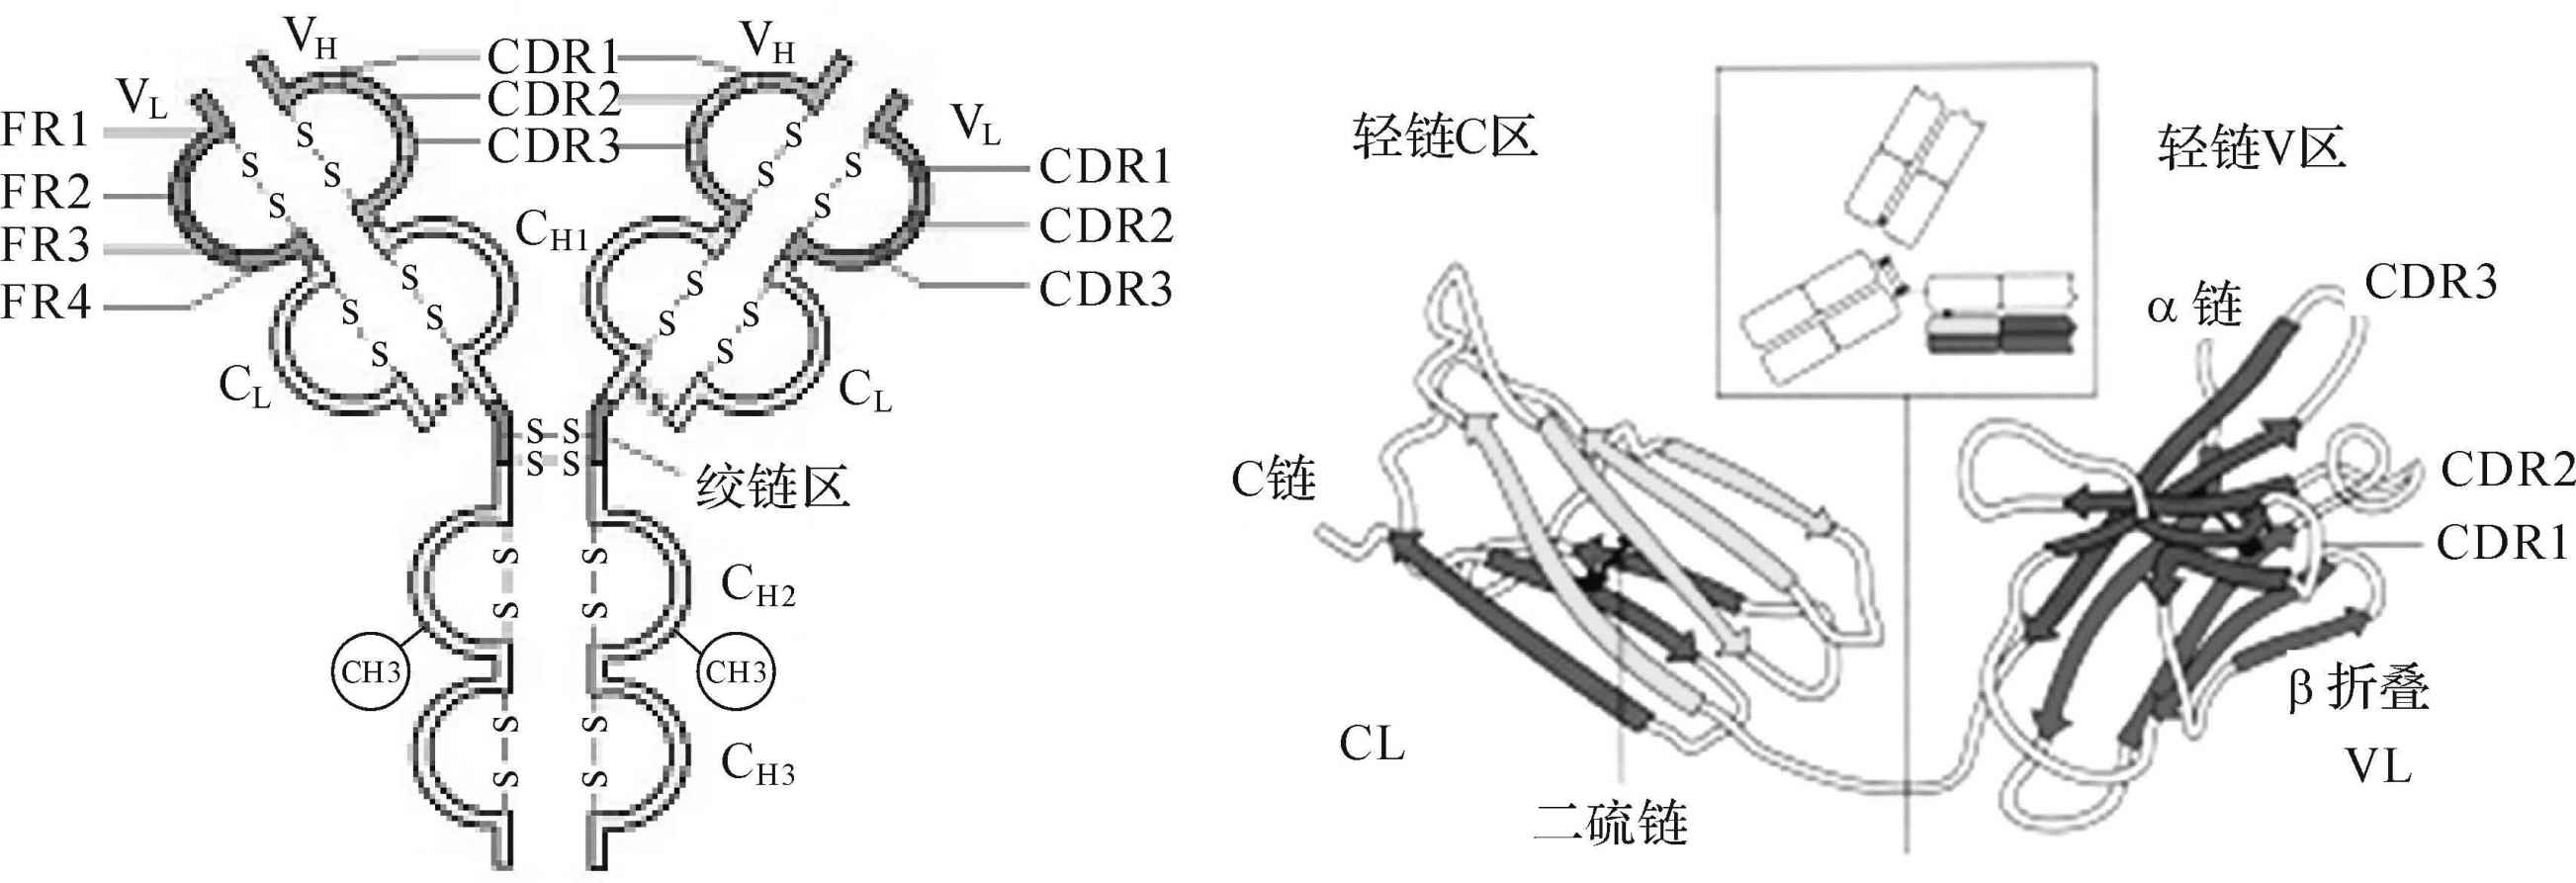
\includegraphics[width=0.7\textwidth]{./images/Image00063.jpg}
 \captionsetup{justification=centering}
 \caption{免疫球蛋白功能区}
 \label{fig4-3}
  \end{figure} 

重链和轻链的C区分别称为C\textsubscript{H} 和C\textsubscript{L}
,不同型(κ或λ)Ig其CL的长度基本一致,但不同类Ig其C\textsubscript{H}
的长度不一,可包括C\textsubscript{H} 1~C\textsubscript{H}
3或C\textsubscript{H} 1~C\textsubscript{H}
4。同一种属的个体,所产生针对不同抗原的同一类别Ig,其C区氨基酸组成和排列顺序比较恒定,即免疫原性相同,但V区各异。Ig
C区与抗体的生物学效应相关,如激活补体;穿过胎盘和黏膜屏障;结合细胞表面Fc受体从而介导调理作用;介导ADCC作用和I型超敏反应等。

(三)绞链区

绞链区位于C\textsubscript{H} 1与C\textsubscript{H}
2之间。该区富含脯氨酸而易伸展弯曲,能改变两个Y形臂之间的距离,有利于两臂同时结合两个不同的抗原表位。IgD、IgG、IgA有绞链区,IgM和IgE则无。

(四)功能区或结构域

免疫球蛋白分子的两条重链和两条轻链都可折叠为数个环形结构域。每个结构域一般具有其独特的功能,因此又称为功能区(domain)。每个功能区约含110个氨基酸残基,其二级结构是由几股多肽链折叠而成的两个反向平行的β片层(anti-parallel
b
sheet),两个β片层中心的两个半胱氨酸残基由一个链内二硫键垂直连接,形成一“β桶状(βbarrel)”结构,或称β三明治(βsandwich)结构。不仅免疫球蛋白,已发现许多膜型和分泌型分子含有这种独特的桶状结构,这类分子被称为免疫球蛋白超家族(immunoglobulin
superfamily,IgSF)。


\subsection{其他成分}

除轻链和重链外,某些类别Ig还含有其他辅助成分,分别是J链(joining
chain)和分泌片(secretory
piece,SP)。J链是一富含半胱氨酸的多肽链,由浆细胞合成,主要功能是将单体Ig分子连接为多聚体。IgA二聚体和IgM五聚体均含J链;IgG、IgD和IgE常为单体,无J链。SP又称分泌成分(secretory
component,SC),为一含糖肽链,由黏膜上皮细胞合成和分泌,以非共价形式结合于IgA二聚体上,使其成为分泌型IgA(SIgA)。SP的作用是:使IgA分泌到黏膜表面,发挥黏膜免疫作用;可保护SIgA绞链区,使其免遭蛋白水解酶降解。


\subsection{Ig水解片段}

在一定条件下,免疫球蛋白分子肽链的某些部分易被蛋白酶水解为各种片段(图\ref{fig4-4})。

\begin{figure}[!htbp]
 \centering
 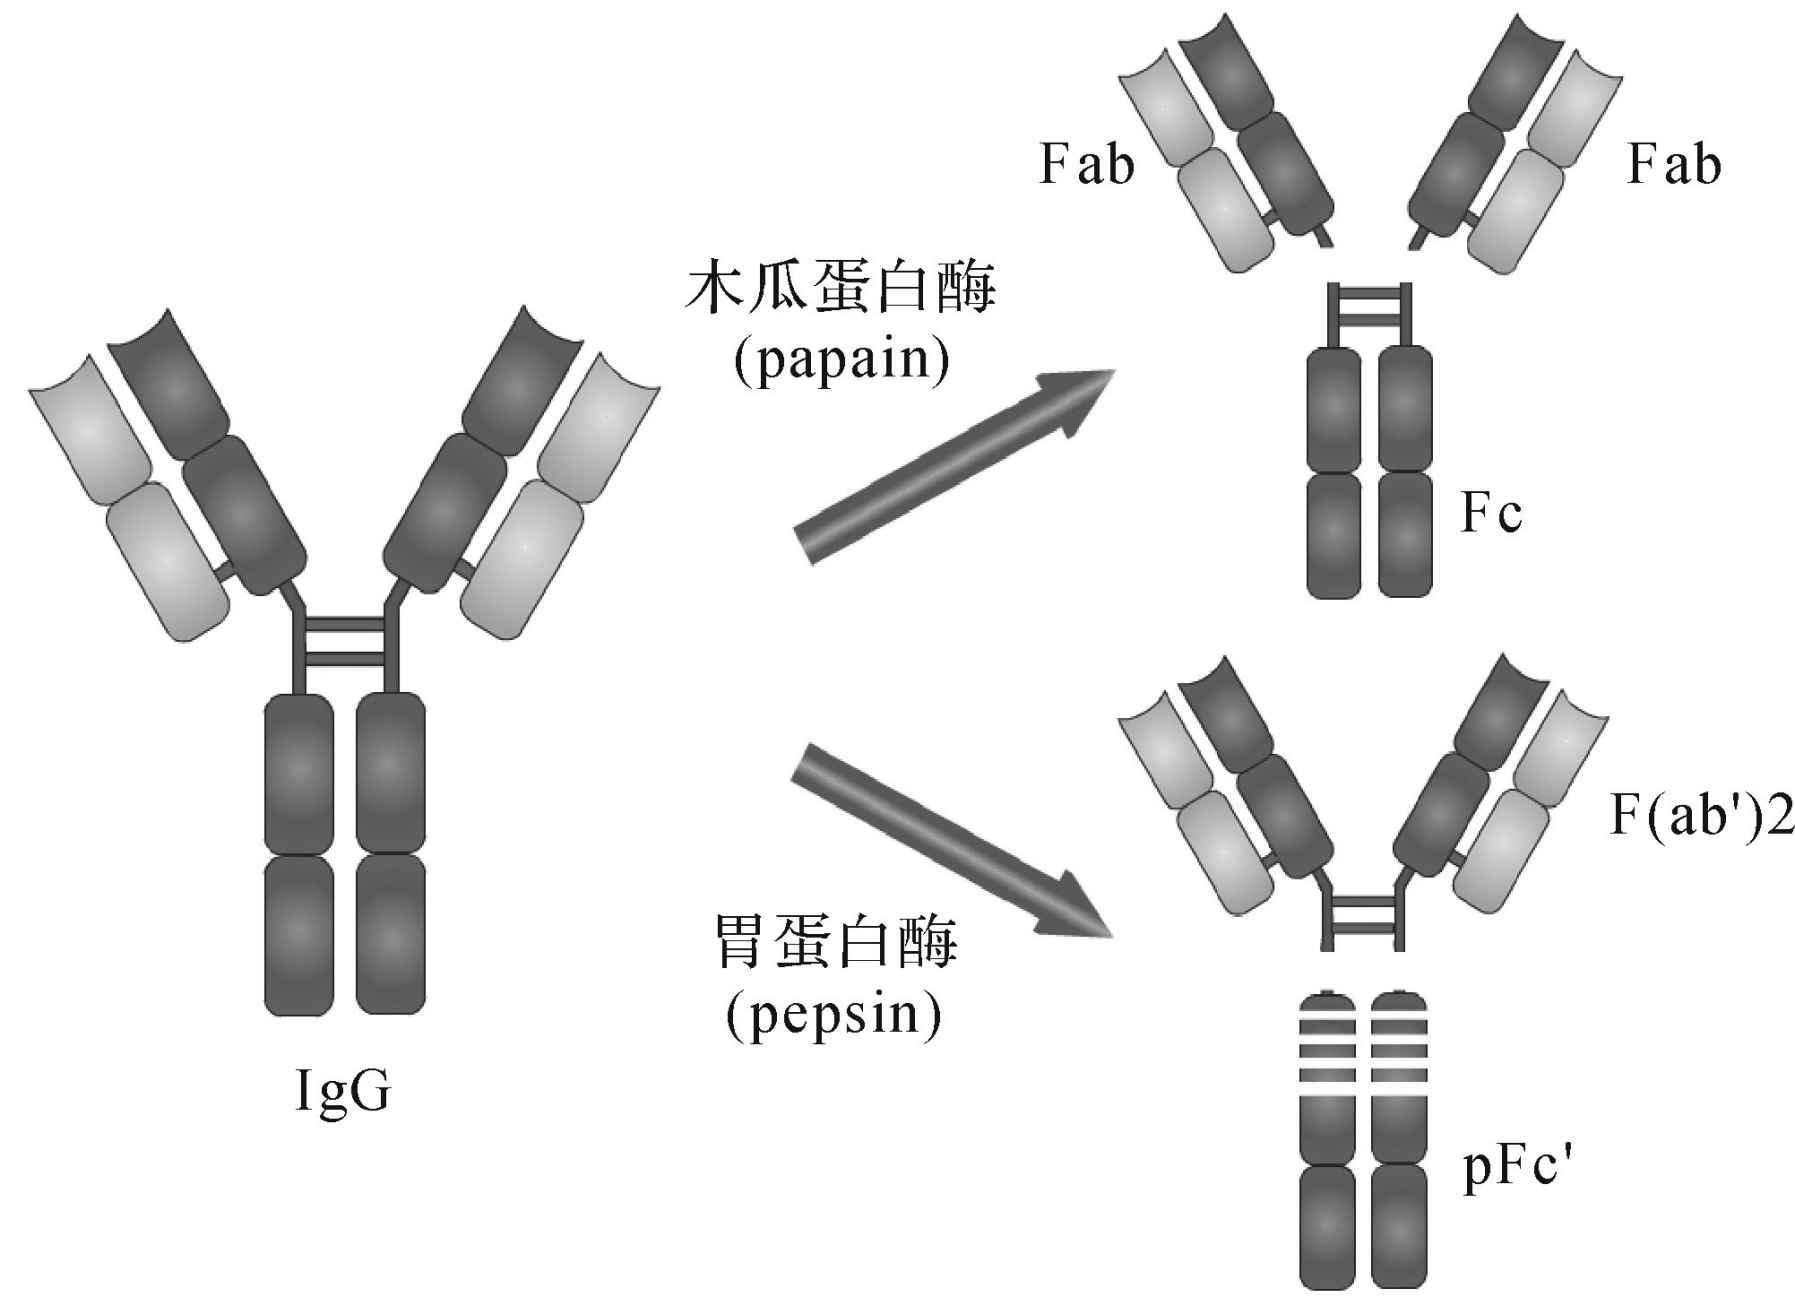
\includegraphics{./images/Image00064.jpg}
 \captionsetup{justification=centering}
 \caption{免疫球蛋白水解示意图}
 \label{fig4-4}
  \end{figure} 

1.木瓜蛋白酶(papain)作用于绞链区二硫键所连接的两条重链的近N端,将Ig裂解为两个完全相同的Fab段和一个Fc段。

(1)Fab即抗原结合片段 (fragment of antigen
binding),由一条完整的轻链和部分重链(V\textsubscript{H}
和C\textsubscript{H}
1)组成。一个Fab片段为单价,可与抗原结合但不形成凝集反应或沉淀反应;因V区的Aa种类、排列顺序、其空间结构具有高度可变性和复杂性,能充分适应Ag决定簇的多样性,也为Ab的多样性和特异性作出了圆满的解释(图\ref{fig4-5})。

\begin{figure}[!htbp]
 \centering
 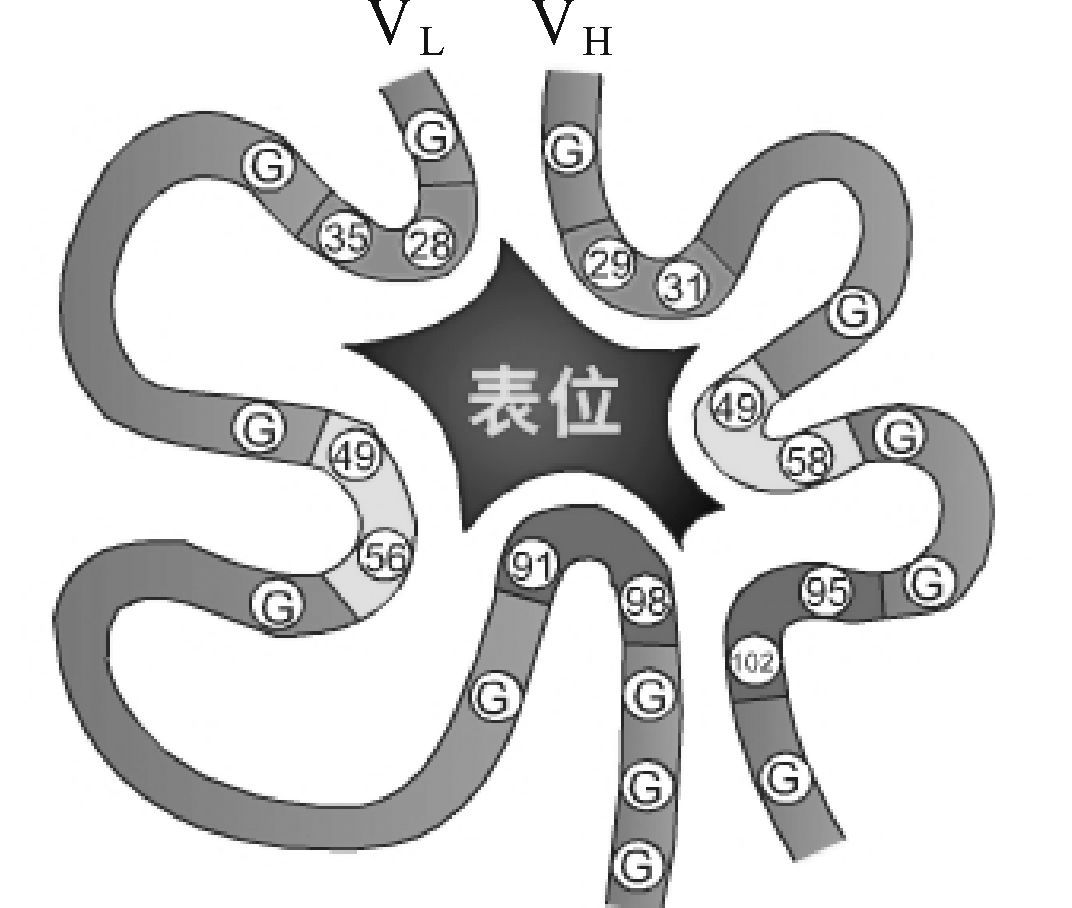
\includegraphics{./images/Image00065.jpg}
 \captionsetup{justification=centering}
 \caption{抗原结合片段}
 \label{fig4-5}
  \end{figure} 

(2)Fc片段即可结晶片段(fragment
crystallizable),相当于IgG的C\textsubscript{H} 2和C\textsubscript{H}
3功能区,无抗原结合活性,是Ig与效应分子或细胞相互作用的部位,与Ig
的生物学活性有关。如:激活补体,增强巨噬细胞的吞噬效果,激活K细胞的杀伤作用。

2.胃蛋白酶(pepsin)作用于绞链区二硫键所连接的两条重链的近C端,将Ig水解为一个大片段F(ab')2和一些小片段pFc'。
F(ab')2是由两个Fab及绞链区组成,为双价,可同时结合两个抗原表位,故能形成凝集反应或沉淀反应。pFc'最终被降解,无生物学作用。

\section{免疫球蛋白的生物学活性}


\subsection{与相应抗原特异性结合}

1.IgV区的氨基酸构型与相应决定簇的立体构型互相吻合。

2.Ig(负电荷)与Ag(正电荷)相互吸引。

3.Ig与Ag相互形成氢键。


\subsection{激活补体}

IgG和IgM与相应抗原结合后,可因构型改变而使其C\textsubscript{H}
2/C\textsubscript{H}
3功能区内的补体结合点暴露,从而激活补体经典途径。IgA和IgE的凝聚物可激活补体旁路途径(图\ref{fig4-6})。

\begin{figure}[!htbp]
 \centering
 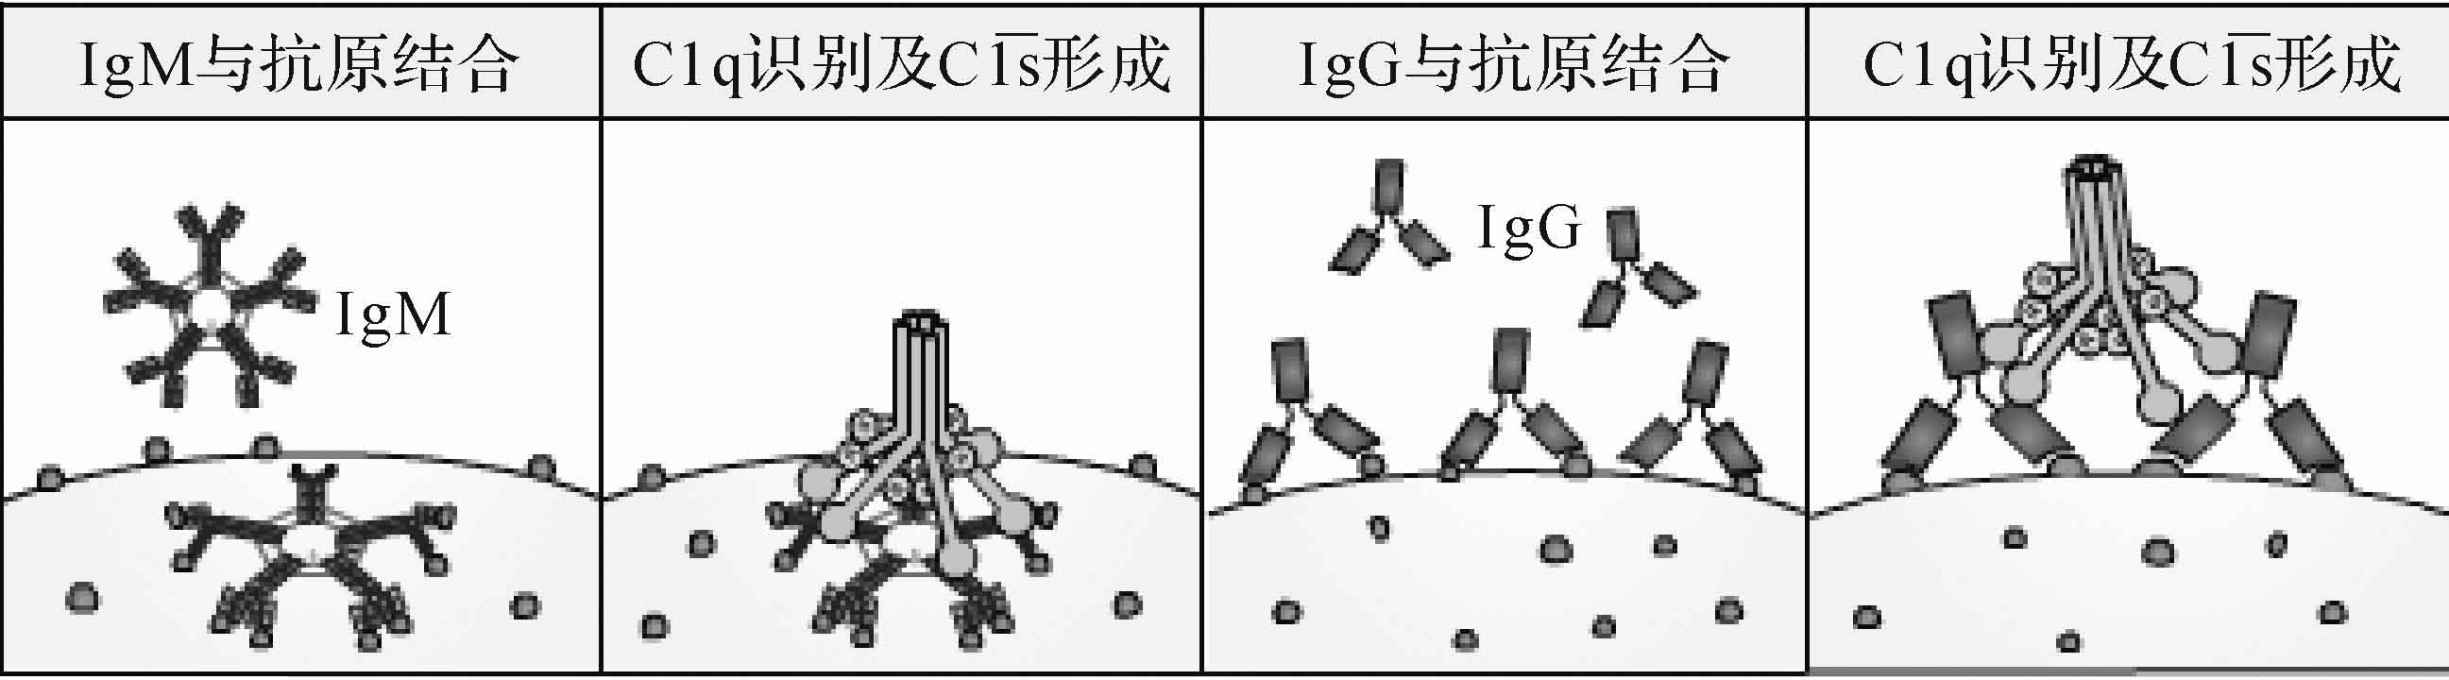
\includegraphics{./images/Image00066.jpg}
 \captionsetup{justification=centering}
 \caption{激活补体}
 \label{fig4-6}
  \end{figure} 


\subsection{结合细胞,产生多种生物学效应}

1.调理作用:
IgG与细菌等颗粒性抗原结合后,可通过其Fc段与巨噬细胞和中性粒细胞表面相应IgG
Fc受体结合,促进吞噬细胞对细菌等颗粒抗原的吞噬(图\ref{fig4-7})。

\begin{figure}[!htbp]
 \centering
 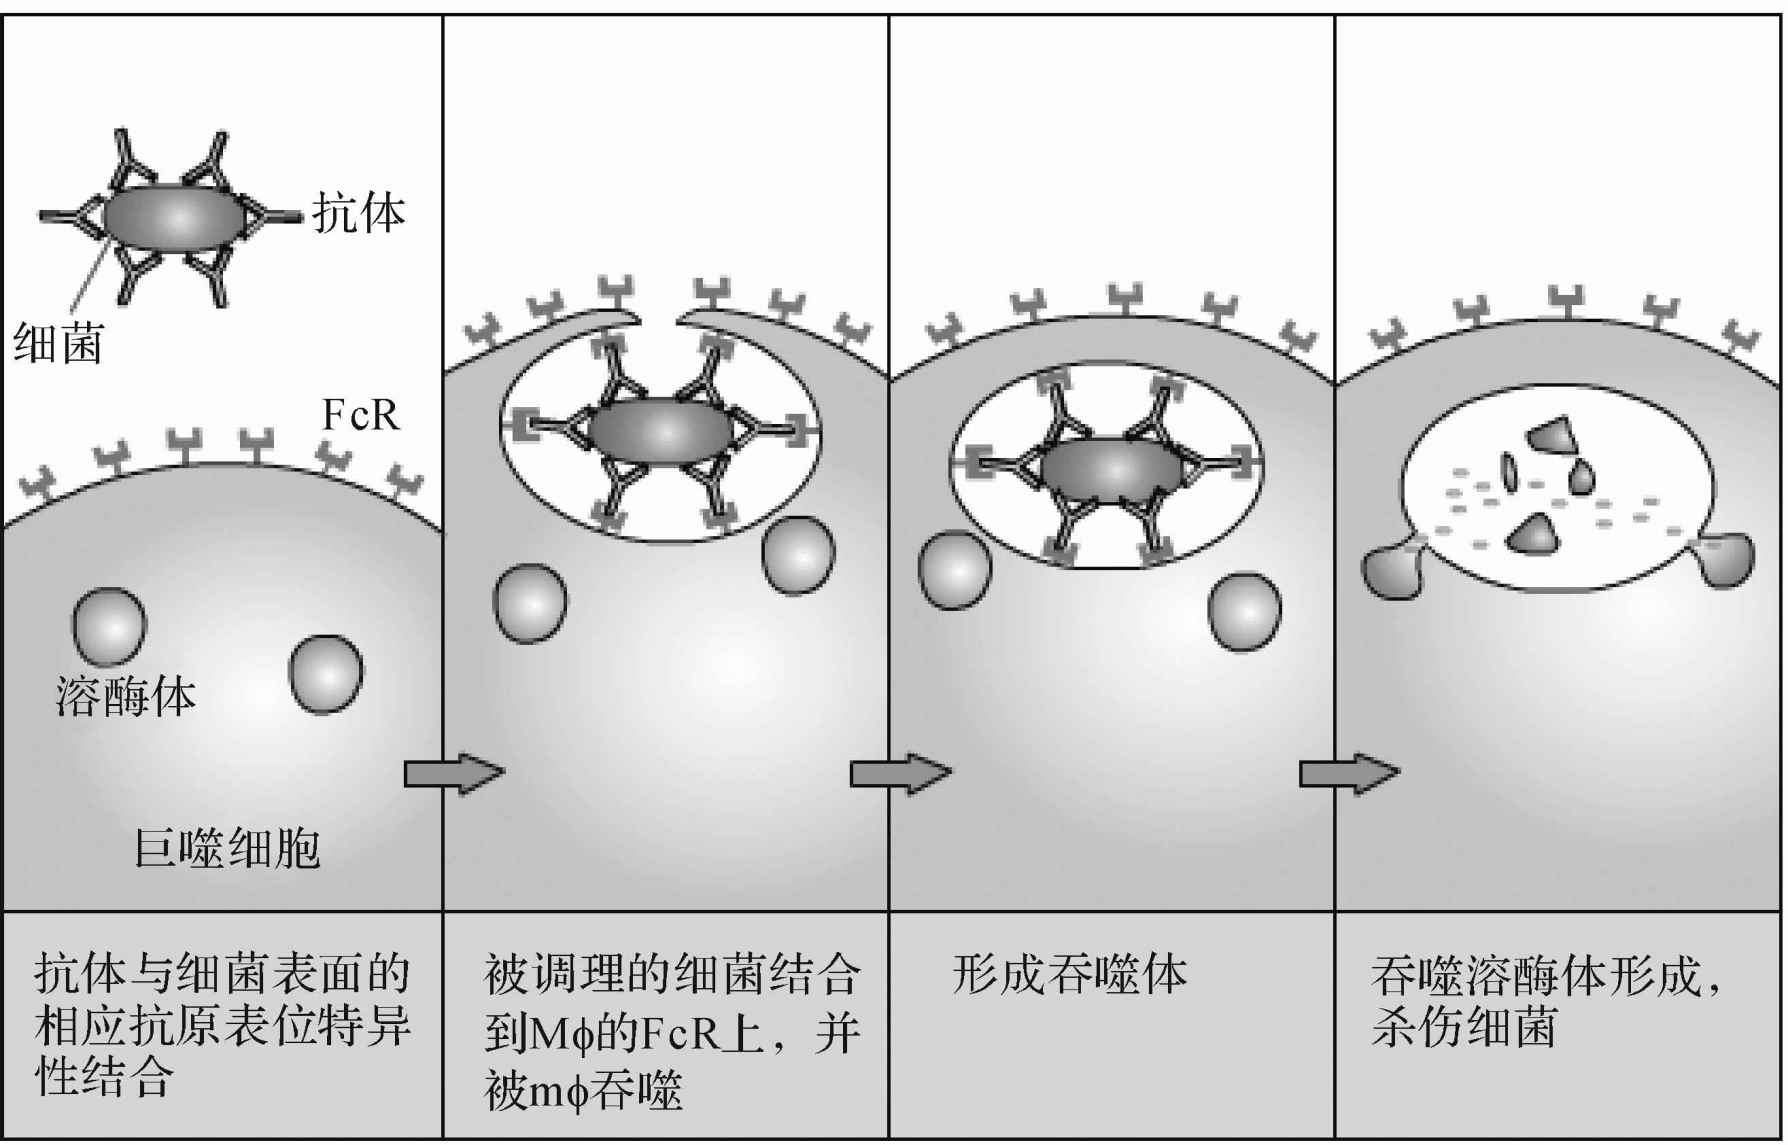
\includegraphics{./images/Image00067.jpg}
 \captionsetup{justification=centering}
 \caption{调理作用}
 \label{fig4-7}
  \end{figure} 

2.抗体依赖细胞介导的细胞毒作用(antibody dependent cell-mediated
cytotoxicity,ADCC):IgG与肿瘤或病毒感染的靶细胞结合后,可通过其Fc段与NK细胞、巨噬细胞和中性粒细胞表面相应IgG
Fc受体结合,增强NK细胞和触发吞噬细胞对靶细胞的杀伤作用(图\ref{fig4-8})。

\begin{figure}[!htbp]
 \centering
 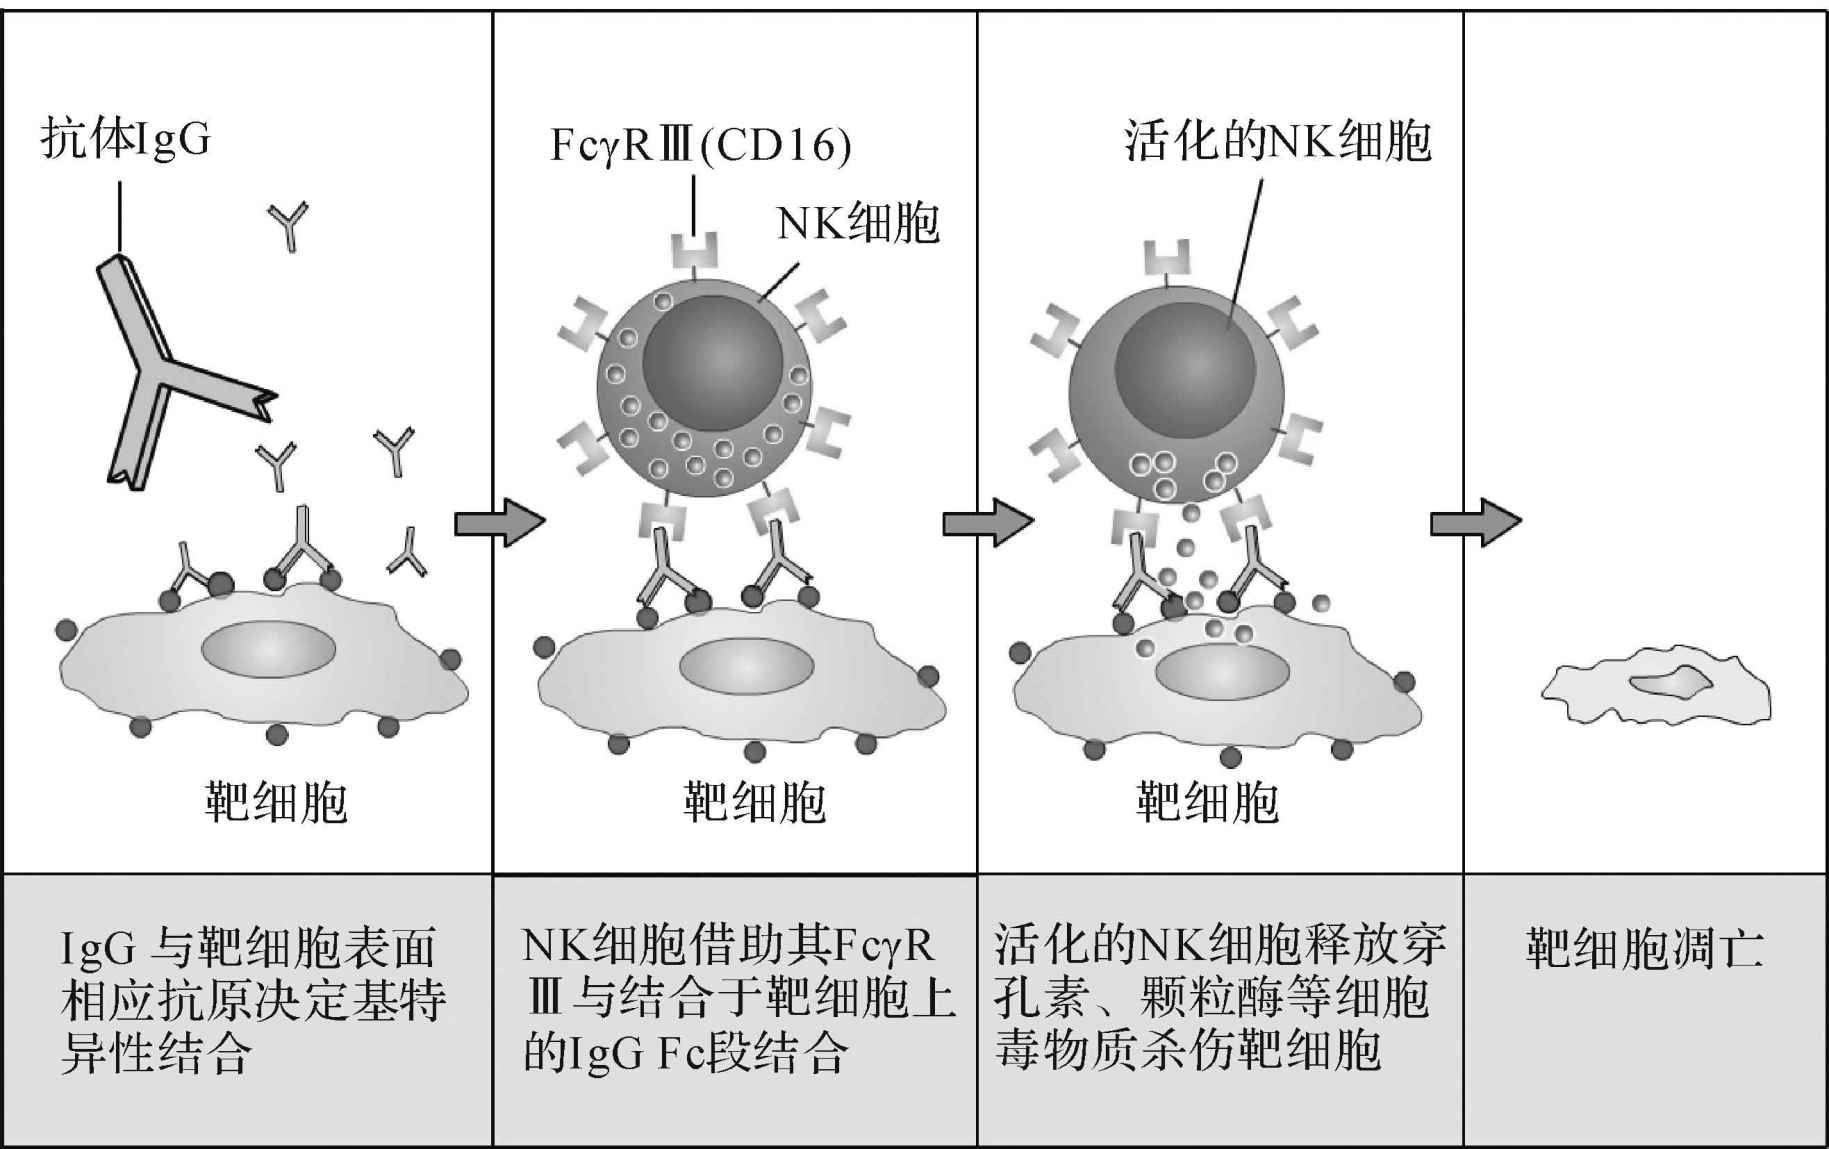
\includegraphics{./images/Image00068.jpg}
 \captionsetup{justification=centering}
 \caption{NK细胞介导的ADCC作用}
 \label{fig4-8}
  \end{figure} 

3.介导I型超敏反应:IgE为亲细胞抗体,可通过其Fc段与肥大细胞和嗜碱粒细胞表面相应IgE
Fc受体结合,而使上述细胞致敏。若相同变应原再次进入机体与致敏靶细胞表面特异性IgE结合,即可使之脱颗粒,释放组胺等生物活性介质,引起I型超敏反应(图\ref{fig4-9})。

\begin{figure}[!htbp]
 \centering
 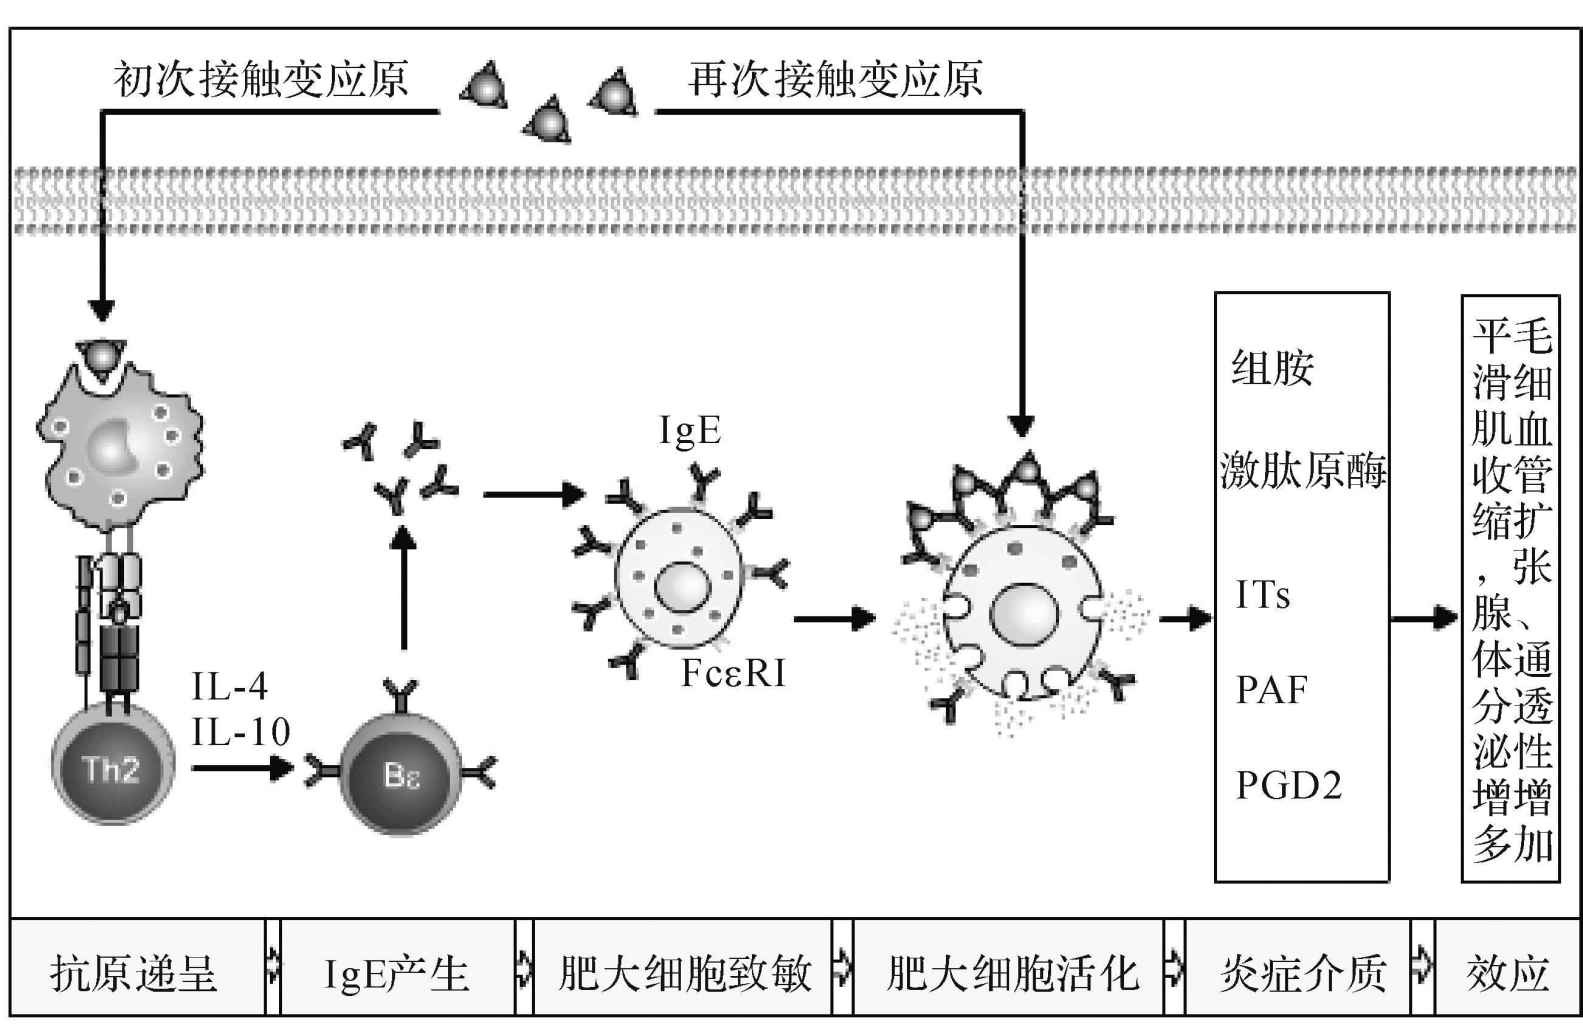
\includegraphics[width=0.6\textwidth]{./images/Image00069.jpg}
 \captionsetup{justification=centering}
 \caption{I型超敏反应示意图}
 \label{fig4-9}
  \end{figure} 


\subsection{通过胎盘被动免疫}

IgG是唯一能从母体转移到胎儿体内的Ig,有增强胎儿、新生儿抗感染作用。

免疫球蛋白的生物学活性如图\ref{fig4-10}所示。

\begin{figure}[!htbp]
 \centering
 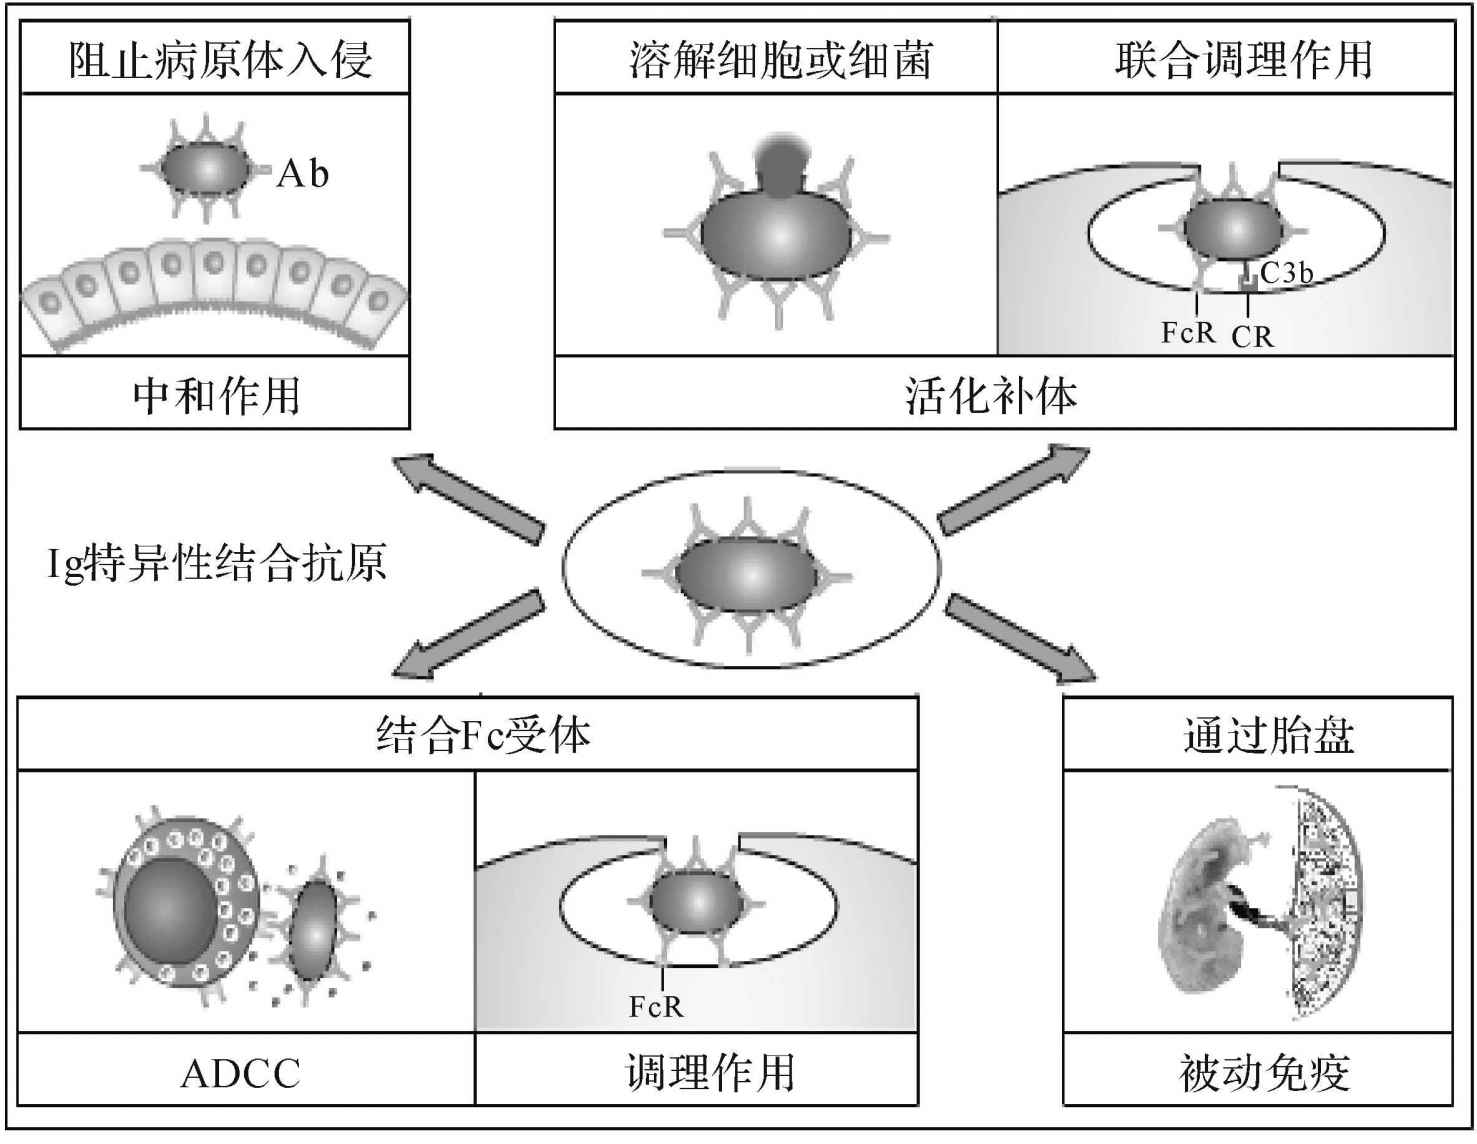
\includegraphics{./images/Image00070.jpg}
 \captionsetup{justification=centering}
 \caption{免疫球蛋白的生物学活性}
 \label{fig4-10}
  \end{figure} 

\section{各类免疫球蛋白的生物学活性}


\subsection{IgG}

IgG是血清和胞外液中主要的抗体成分,约占血清免疫球蛋白总量的80%。按照其绞链区大小以及链内二硫键数目和位置的不同,可将人IgG分为4个亚类,依其在血清中浓度高低,分别为IgG1、IgG2、IgG3、IgG4。IgG自出生后3个月开始合成,3~5岁接近成人水平。IgG的半衰期为20~23天,是再次体液免疫应答产生的主要抗体,其亲和力高,在体内分布广泛,具有重要的免疫效应,是机体抗感染的“主力军”。IgG1、IgG3、IgG4可穿过胎盘屏障,在新生儿抗感染免疫中起重要作用;IgG1、IgG2、IgG4可通过其Fc段与葡萄球菌蛋白A(SPA)结合,借此可纯化抗体,并用于免疫诊断;IgG1、IgG3可高效激活补体,并可与巨噬细胞、NK细胞表面Fc受体结合,发挥调理作用、ADCC作用等;某些自身抗体和引起II、III型超敏反应的抗体也属IgG。


\subsection{IgM}

IgM占血清免疫球蛋白总量的5\%~10%,血清浓度约1mg/ml。单体IgM以膜结合型(mIgM)表达于B细胞表面,构成B细胞抗原受体(BCR);分泌型IgM为五聚体,不能通过血管壁,主要存在于血清中。五聚体IgM含10个Fab段,具有很强的抗原结合能力;含5个Fc段,比IgG更易激活补体。天然血型抗体为IgM,血型不符的输血可致严重溶血反应。IgM是个体发育中最早合成的抗体,脐带血IgM升高提示胎儿宫内感染;IgM也是初次体液免疫应答中最早出现的抗体,是机体抗感染的“先头部队”;血清中检出IgM,提示新近发生感染,可用于感染的早期诊断。


\subsection{IgA}

IgA仅占血清免疫球蛋白总量的10\%~15%,但却是外分泌液中的主要抗体类别。IgA分为两型:血清型为单体,主要存在于血清中;分泌型IgA(secretory
IgA,SIgA)为二聚体,由J链连接,含内皮细胞合成的SP,经分泌性上皮细胞分泌至外分泌液中。

SP的主要功能是介导IgA穿过上皮细胞腺体腔或黏膜表面,其机制为:SP作为受体与IgA结合,形成永久性共价复合物SIgA。SIgA主要存在于乳汁、唾液、泪液和呼吸道、消化道、生殖道黏膜表面,参与局部的黏膜免疫。新生儿易患呼吸道、消化道感染,可能与其SIgA合成不足有关。婴儿可从母乳中获得SIgA,属重要的自然被动免疫。


\subsection{IgD}

IgD仅占血清免疫球蛋白总量的0.2%,血清浓度约30ug/ml。在五类Ig中,IgD的绞链区较长,易被蛋白酶水解,故其半衰期较短(仅3天)。IgD分为两型:血清IgD的生物学功能尚不清楚;膜结合型IgD(mIgD)构成BCR,是B细胞分化成熟的标志。未成熟B细胞仅表达mIgM;成熟B细胞同时表达mIgM和
mIgD,被称为初始B细胞 (Naive B
cell);活化的B细胞或记忆B细胞其表面的mIgD逐渐消失。


\subsection{IgE}

正常人血清中含量最少的免疫球蛋白是IgE,血清浓度仅为0.3ug/ml,主要由黏膜下淋巴组织中的浆细胞分泌。IgE相对分子量为160kD,其重要特征为糖含量高达12%。IgE具有很强的亲细胞性,其C\textsubscript{H}
2和C\textsubscript{H}
3可与肥大细胞、嗜碱粒细胞表面高亲和力FceRI结合,促使这些细胞脱颗粒并释放生物活性介质,引起I型超敏反应。此外,IgE可能与机体抗寄生虫免疫有关。

图\ref{fig4-11}所示为各类免疫球蛋白结构示意图。

\begin{figure}[!htbp]
 \centering
 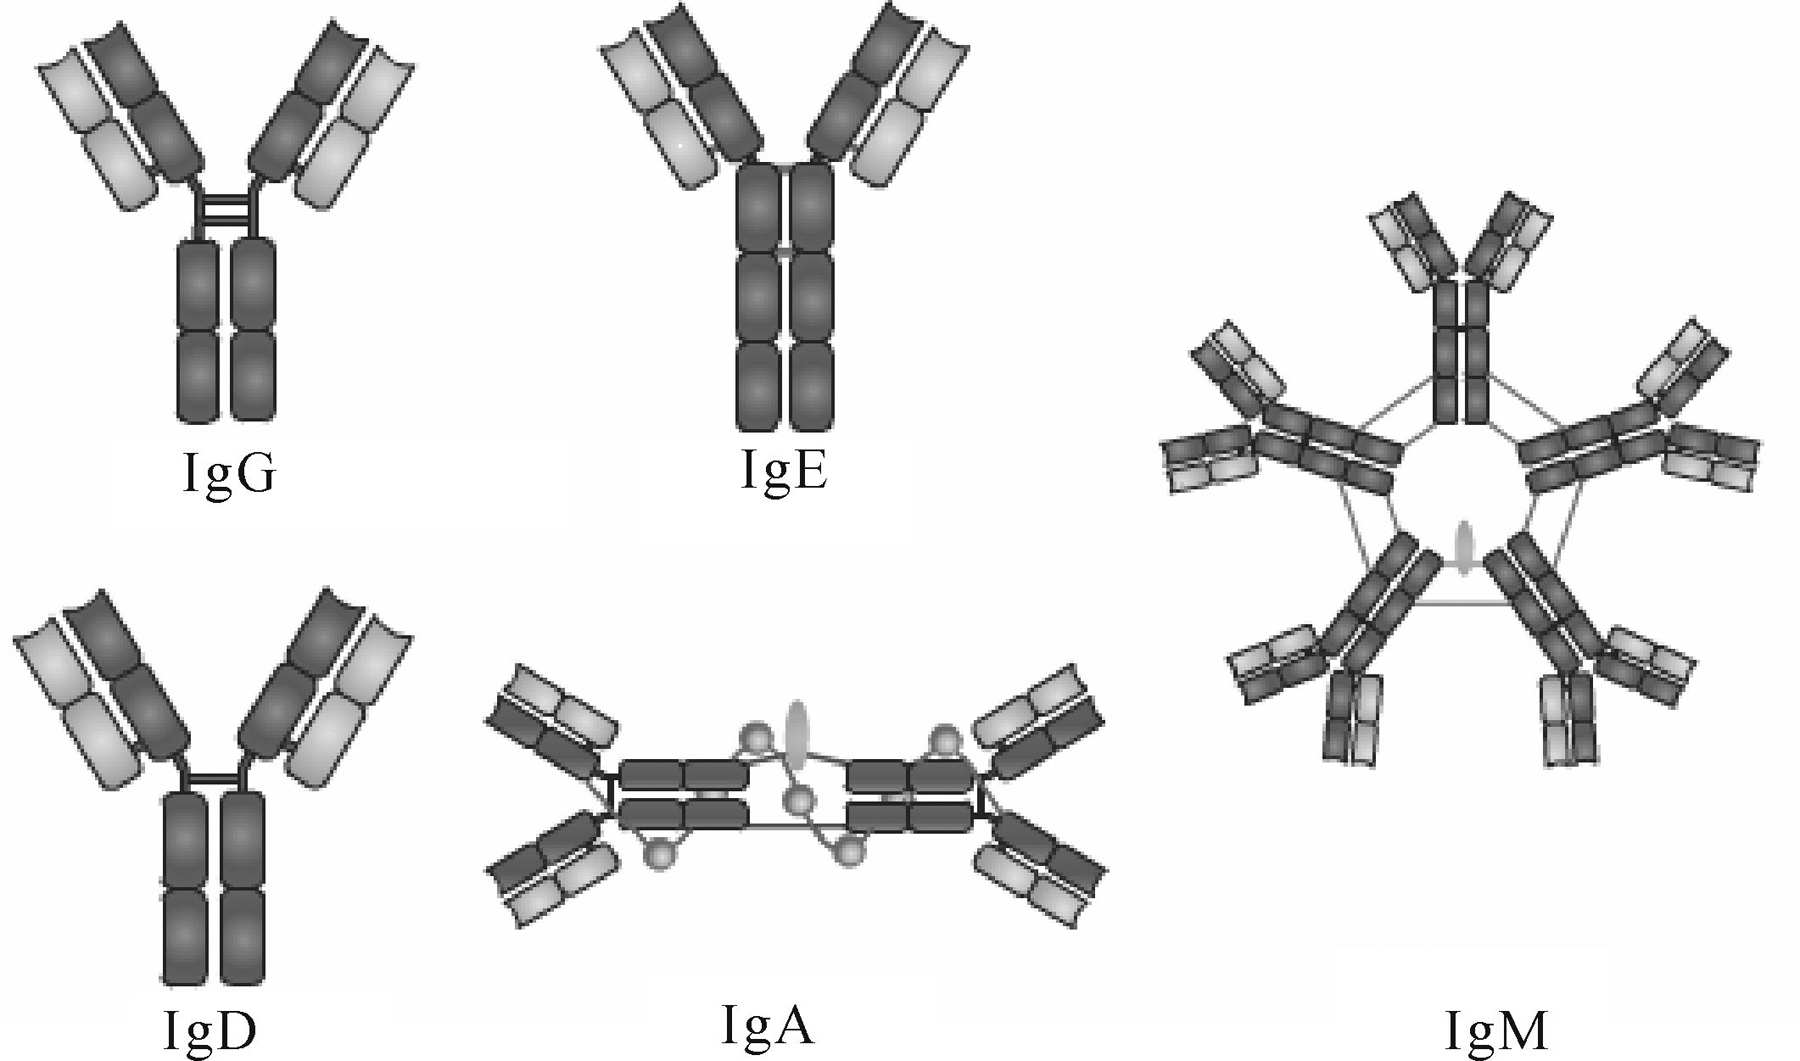
\includegraphics{./images/Image00071.jpg}
 \captionsetup{justification=centering}
 \caption{各类免疫球蛋白}
 \label{fig4-11}
  \end{figure} 

\section{人工制备抗体}

抗体在疾病诊断和免疫防治中发挥重要作用,故对抗体的需求越来越大。人工制备抗体是大量获得抗体的重要途径。早年人工制备抗体的方法主要是以相应抗原免疫动物,获得抗血清。由于天然抗原常含多种不同抗原表位,同时抗血清也未经免疫纯化,故所获抗血清是含多种抗体的混合物,即多克隆抗体
(polyclonal
antibody)。用于制备抗血清的动物由早期的小鼠、大鼠、兔、羊等小动物发展到马等大动物,但所获抗体的质与量均不敷现代医学生物学实践之需。

1975年,Kohler和Milstein建立了体外细胞融合技术,获得免疫小鼠脾细胞与恶性浆细胞瘤细胞融合的杂交瘤细胞,从而使得规模化制备高特异性、均质性的单克隆抗体
(monoclonal antibody,McAb)成为可能。


\subsection{多克隆抗体}

\begin{figure}[!htbp]
 \centering
 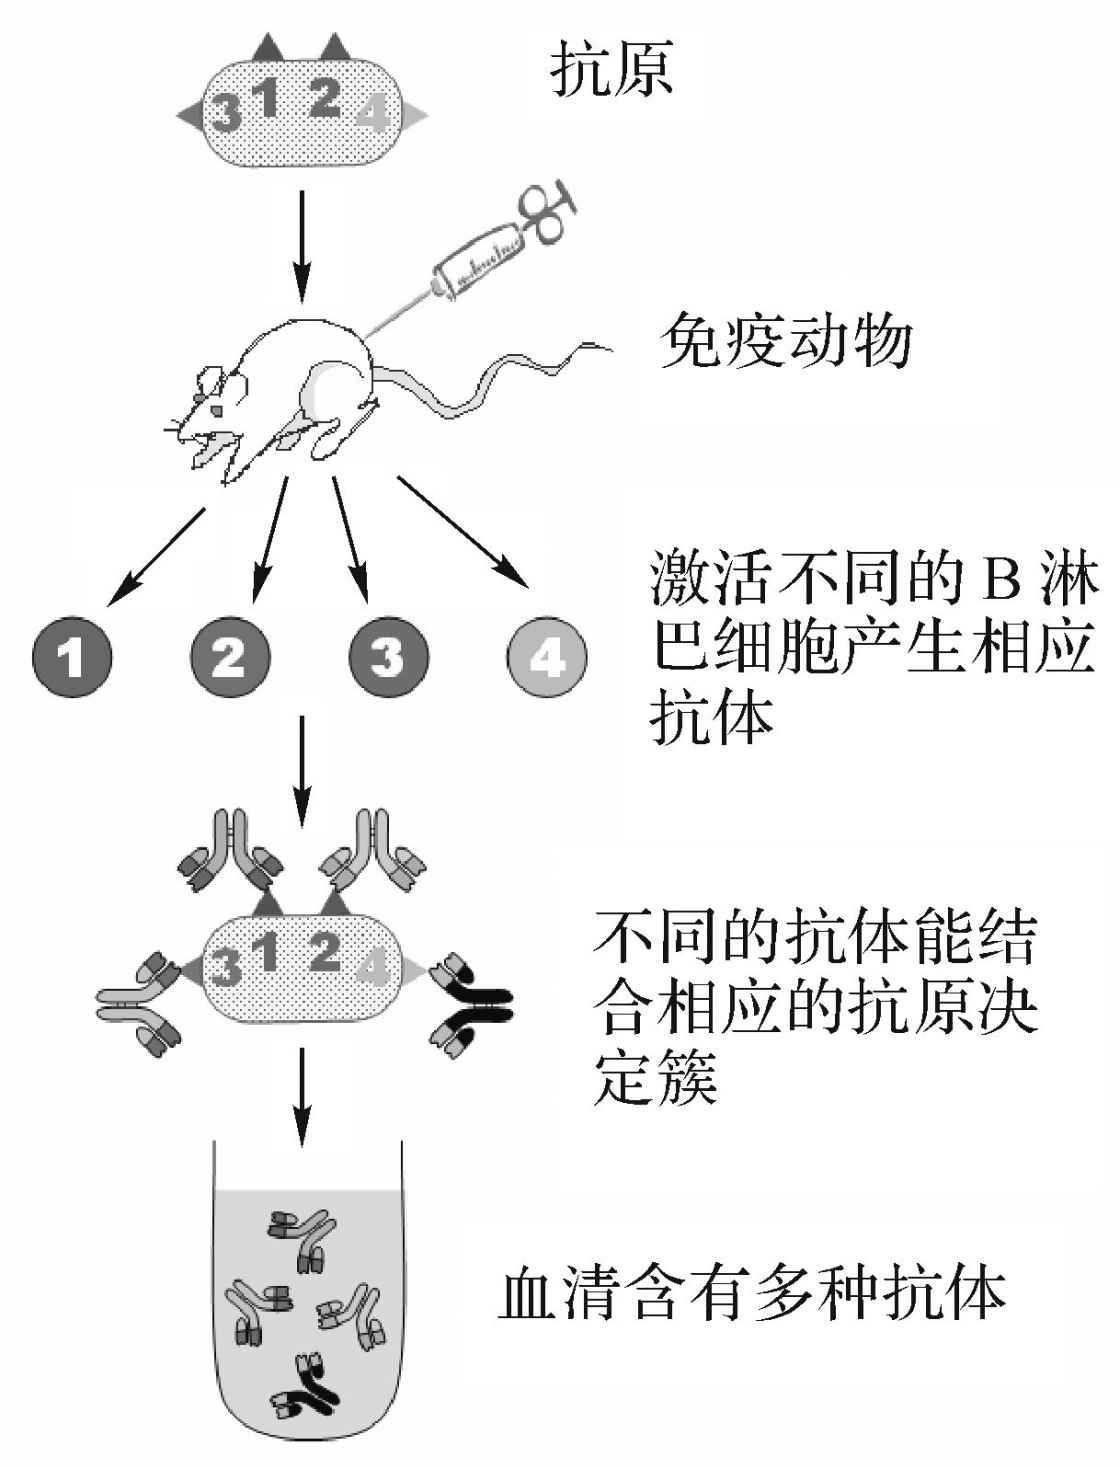
\includegraphics{./images/Image00072.jpg}
 \captionsetup{justification=centering}
 \caption{多克隆抗体制备示意图}
 \label{fig4-12}
  \end{figure} 

在含多种抗原表位的抗原物质刺激下,体内多个B细胞克隆被激活并产生针对多种不同抗原表位的抗体,其混合物即为多克隆抗体。多克隆抗体是机体发挥特异性体液免疫效应的关键分子,具有中和抗原、免疫调理、介导CDC、ADCC等重要作用。在体外,多克隆抗体主要来源于动物免疫血清、恢复期病人血清或免疫接种人群。其特点是来源广泛、制备容易。多克隆抗体是针对不同抗原表位的抗体的混合物,而并非仅针对某一特定表位,其缺点是:特异性不高、易发生交叉反应,也不易大量制备,从而应用受限,图\ref{fig4-12}为多克隆抗体制备示意图。


\subsection{单克隆抗体}

制备单一表位特异性抗体的理想方法是获得仅针对单一表位的浆细胞克隆,使其在体外扩增并分泌抗体。然而,浆细胞在体外的寿命较短,也难以培养。为克服此缺点,Kohler和Milstein将可产生特异性抗体但短寿的浆细胞与无抗原特异性但长寿的恶性浆细胞瘤细胞融合,建立了可产生单克隆抗体的杂交瘤细胞和单克隆抗体技术(图\ref{fig4-13})。

\begin{figure}[!htbp]
 \centering
 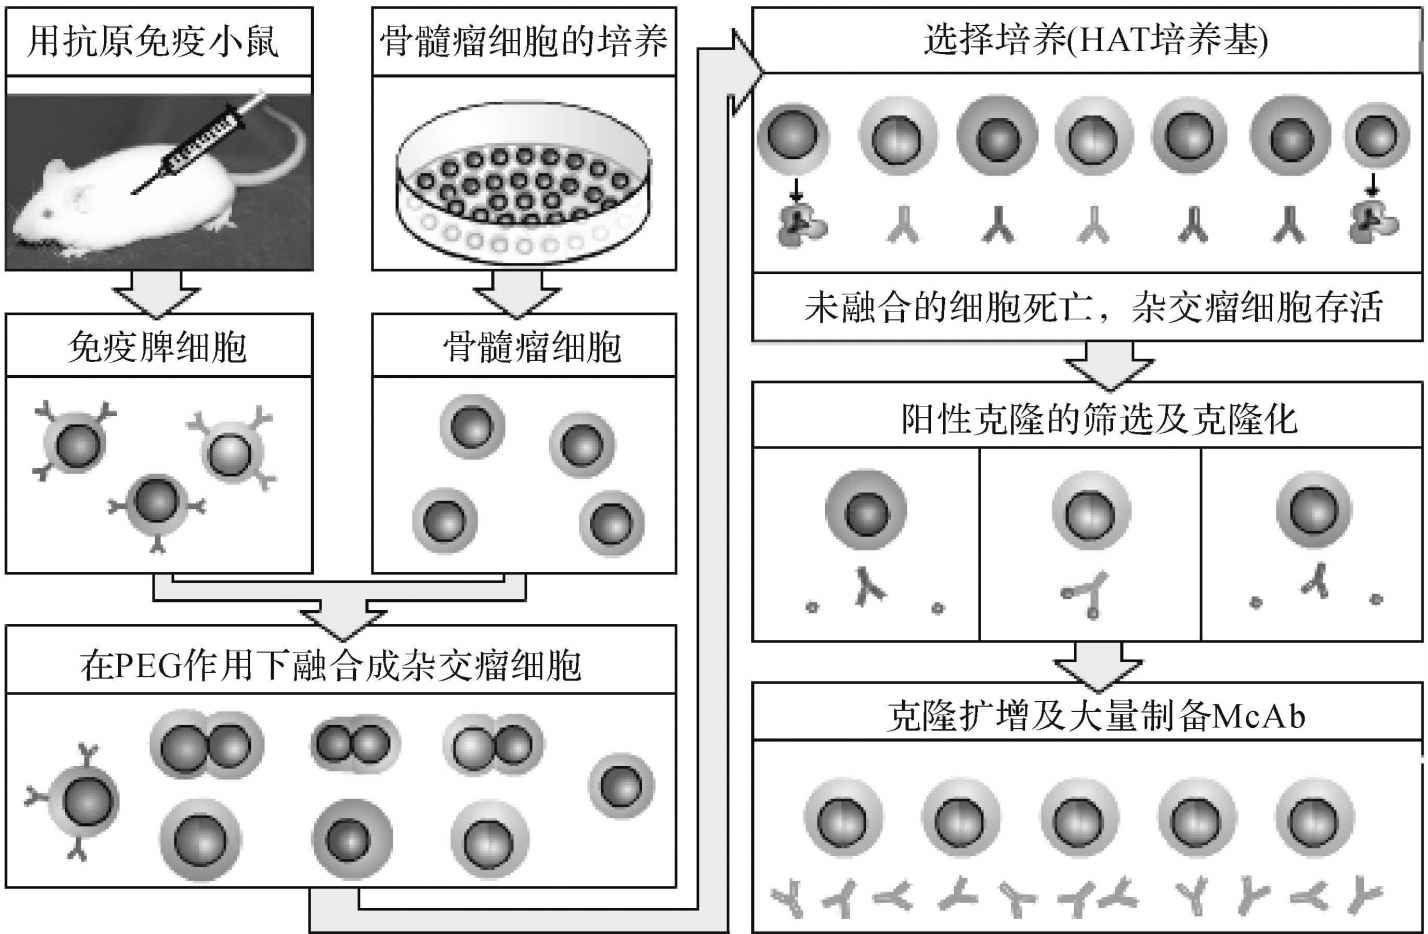
\includegraphics[width=0.6\textwidth]{./images/Image00073.jpg}
 \captionsetup{justification=centering}
 \caption{单克隆抗体的制备}
 \label{fig4-13}
  \end{figure} 

单克隆抗体技术的基本原理是:哺乳类细胞的DNA合成分为从头(do
novo)合成和补救(Salvage)合成两条途径。前者利用磷酸核糖焦磷酸和尿嘧啶,可被氨基喋呤(A)阻断;后者则在次黄嘌呤磷酸核糖转化酶(HGPRT)存在下利用次黄嘌呤(H)和胸腺嘧啶(T);脾细胞和骨髓瘤细胞在聚乙二醇(PEG)作用下可发生细胞融合;加入HAT选择培养基(含H、A和T)后,未融合的骨髓瘤细胞因其从头合成途径被氨基喋呤阻断而又缺乏HGPRT不能利用补救途径合成DNA,因而死亡;未融合的脾细胞因不能在体外培养而死亡;融合细胞因从脾细胞获得HGPRT,故可在HAT选择培养基中存活和增殖。

融合形成的杂交细胞系称为杂交瘤(hybridoma),其既有骨髓瘤细胞大量扩增和永生的特性,又具有免疫B细胞合成和分泌特异性抗体的能力。

单克隆抗体在结构和组成上高度均一,抗原特异性及同种型一致,易于体外大量制备和纯化。因此,其具有纯度高、特异性强、效价高、少或无血清交叉反应、制备成本低等优点,已广泛用于疾病诊断、特异性抗原或蛋白的检测和鉴定、疾病的被动免疫治疗和生物导向药物制备等。


\subsection{基因工程抗体(genetic engineering antibody)}

单克隆抗体问世后,在生命科学理论研究和临床实践中得到极为广泛的应用。但是,迄今所获单克隆抗体多为鼠源性,鼠免疫球蛋白会使机体产生人抗鼠抗体反应,导致被快速清除,半衰期短,需给药次数多、剂量大,鼠抗体可能引起严重过敏反应。如何去除McAb的免疫原性而保留其免疫反应性?理想的方案是McAb只包含人的氨基酸序列,无鼠的氨基酸成分。即按不同的需要,将抗体的基因进行加工、改造和重新装配,然后再导入到适当的受体细胞内进行表达的抗体分子,这也就是第三代抗体。

与单克隆抗体相比,所具有的优点有:

1.通过基因工程技术的改造,可降低甚至消除人体对抗体的排斥反应;

2.基因工程抗体的分子量较小,可部分降低抗体的鼠源性,更加有利于穿透血管壁,进入病灶的核心部位;

3.可采用原核细胞、真核细胞和植物等多种表达方式,大量表达抗体分子,大大降低生产成本。

如人-鼠嵌合抗体(chimeric antibody)、改型抗体(reshaped
antibody)、双特异性抗体(bispecific antibody)、小分子抗体等。

(一)人-鼠嵌合抗体(chimeric antibody)

人-鼠嵌合抗体是将鼠源单抗的可变区与人抗体的恒定区融合而得到的抗体(图\ref{fig4-14})。构建嵌合抗体的大致过程是:将鼠源单抗的可变区基因克隆出来,连到包含有人抗体恒定区基因及表达所需的其他元件(如启动子、增强子、选择标记等)的表达载体上,在哺乳动物细胞(如骨髓瘤细胞、CHO细胞)中表达。

\begin{figure}[!htbp]
 \centering
 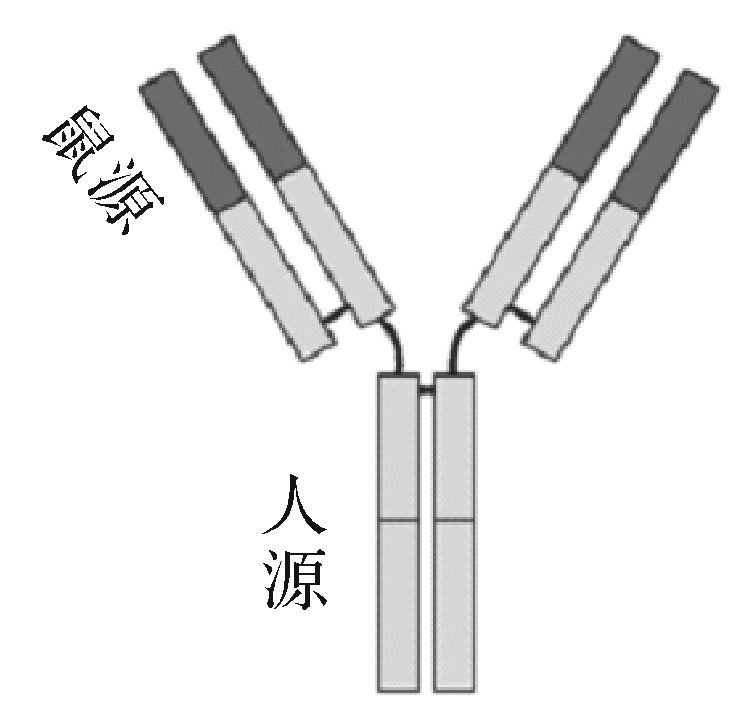
\includegraphics{./images/Image00074.jpg}
 \captionsetup{justification=centering}
 \caption{小鼠嵌合抗体}
 \label{fig4-14}
  \end{figure} 

\begin{figure}[!htbp]
 \centering
 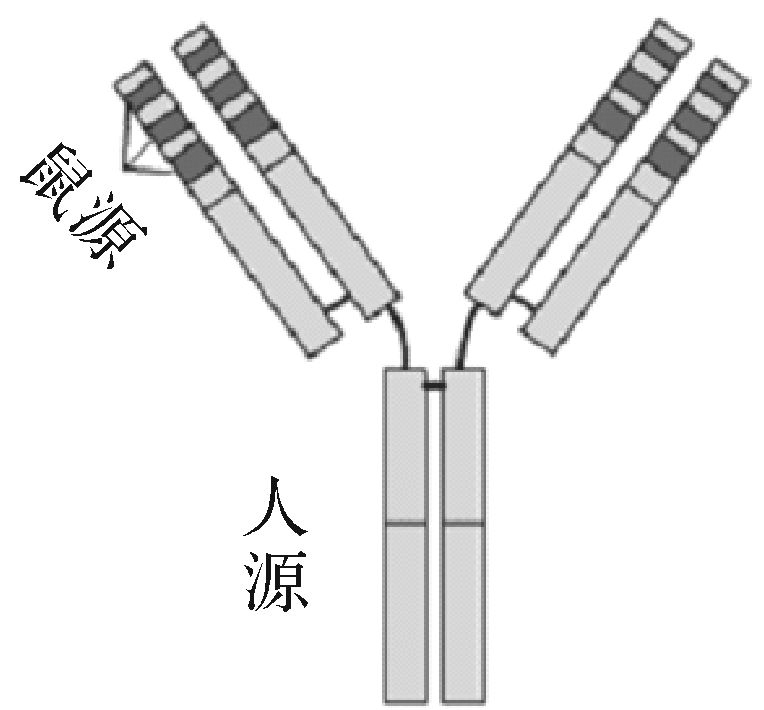
\includegraphics{./images/Image00075.jpg}
 \captionsetup{justification=centering}
 \caption{改型抗体}
 \label{fig4-15}
  \end{figure} 

\begin{figure}[!htbp]
 \centering
 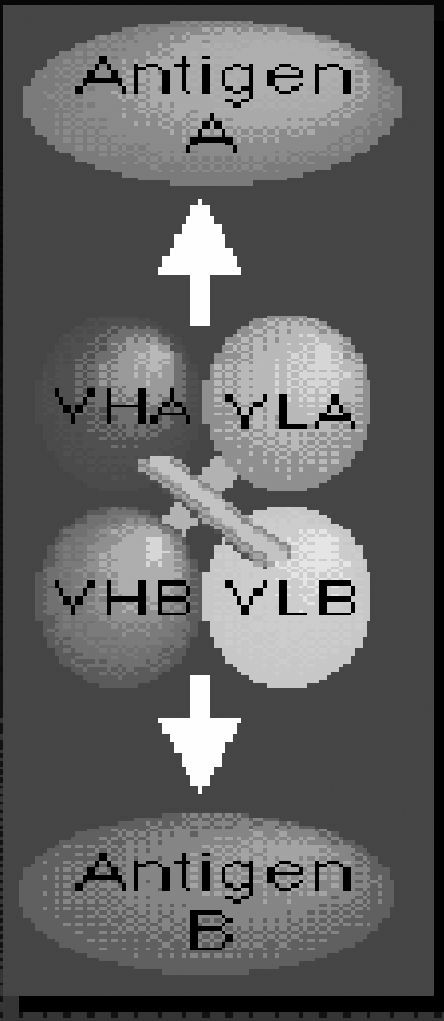
\includegraphics{./images/Image00076.jpg}
 \captionsetup{justification=centering}
 \caption{双特异性抗体}
 \label{fig4-16}
  \end{figure} 

(二)改型抗体或称CDR移植抗体

CDR移植即把鼠抗体的CDR序列移植到人抗体的可变区内,所得到的抗体称CDR移植抗体或改型抗体,也就是人源化抗体(图\ref{fig4-15})。美国正式上市的11种治疗性单抗中多数是改型抗体,优点:(1)特异性较强;(2)不易发生变态反应;(3)在人体内维持的时间较长。

(三)双特异性抗体

双特异性抗体是指能同时识别两种抗原的抗体(图\ref{fig4-16}),一种为对应肿瘤相关抗原,另一种为对应效应成分。即既能结合靶肿瘤细胞又能结合高细胞毒性的效应细胞,将效应细胞富集在肿瘤周围,实现对肿瘤细胞的杀伤和裂解。特点:除了能特异性识别肿瘤细胞外,还能将循环血液中的免疫效应细胞再导向至肿瘤细胞处,从而使效应细胞的抗肿瘤活性增强,发挥免疫导向作用。

(四)小分子抗体

小分子抗体包括Fab、Fv或ScFv、单域抗体及最小识别单位等(图\ref{fig4-17})。小分子抗体有很多优点:可以用细菌发酵生产,成本低;分子小,穿透力强;不含Fc,没有Fc带来的效应;在体内循环的半衰期短,易清除,利于解毒排出;易于与毒素或酶基因连接,便于制备免疫毒素或酶标抗体。

\begin{figure}[!htbp]
 \centering
 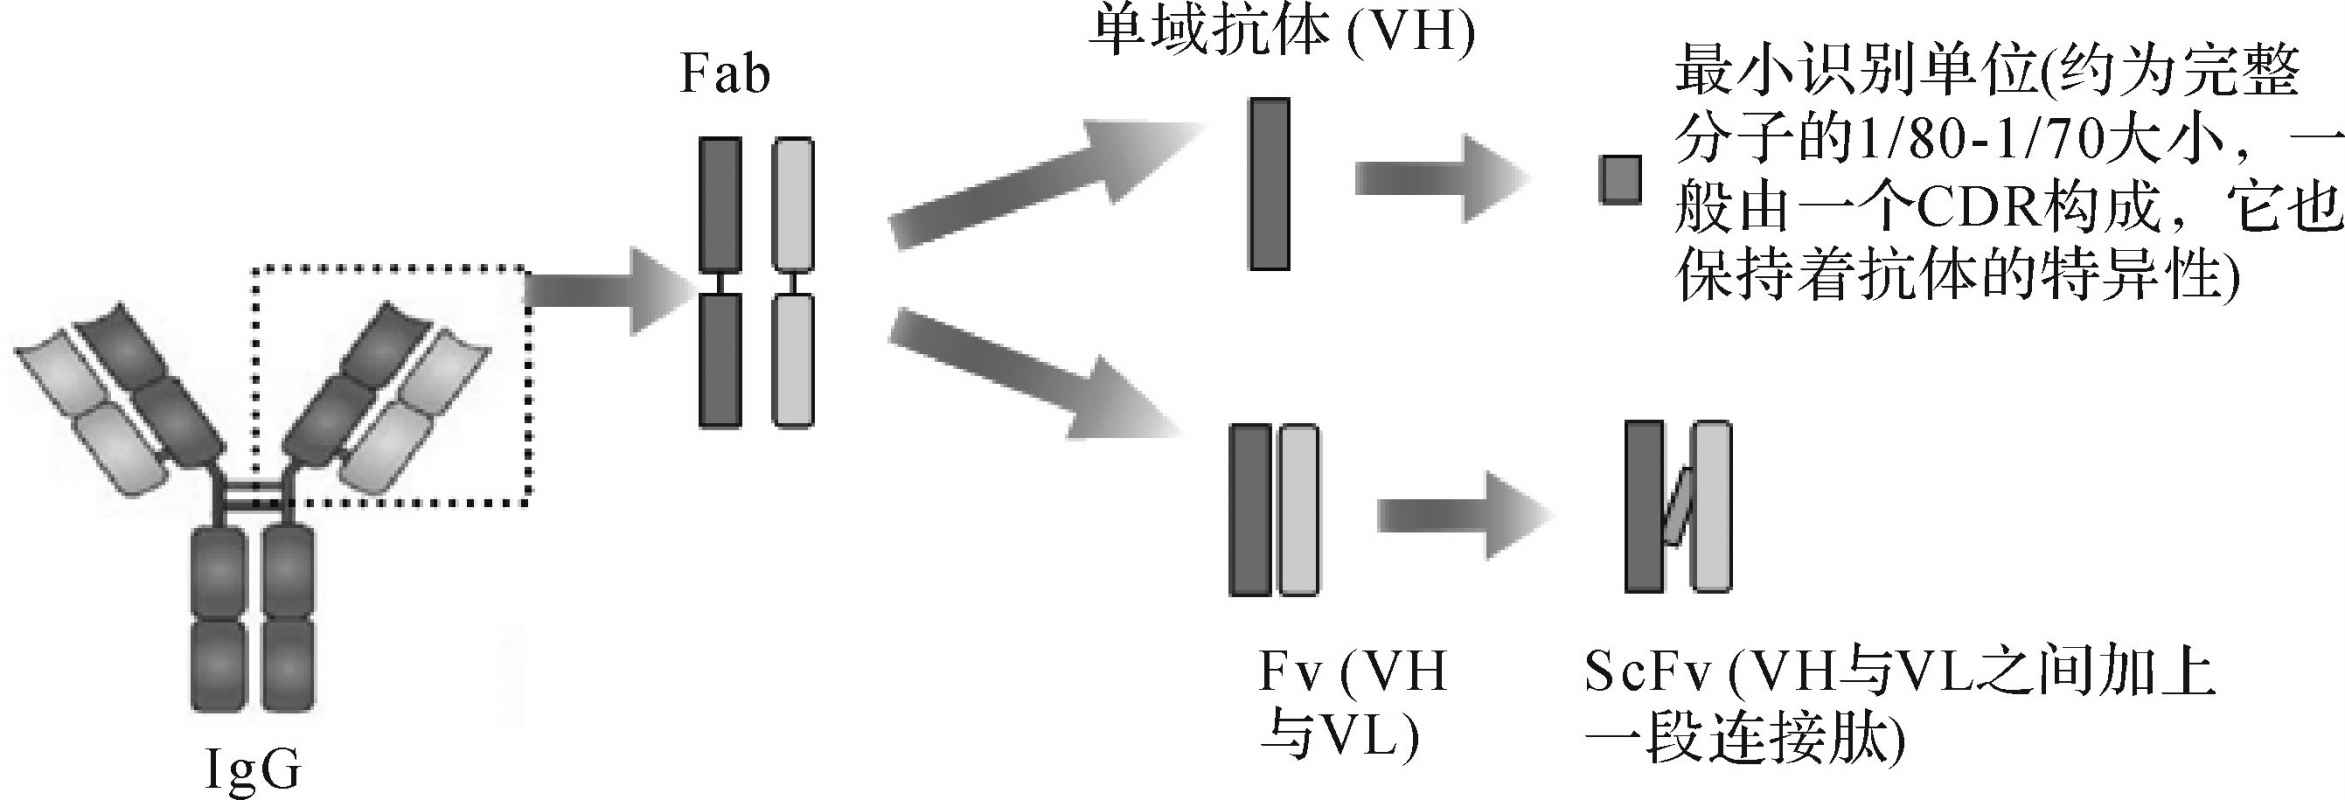
\includegraphics{./images/Image00077.jpg}
 \captionsetup{justification=centering}
 \caption{小分子抗体}
 \label{fig4-17}
  \end{figure} 

\noindent\textbf{【理解与思考】}

1.设想你是免疫球蛋白,向别人介绍你是如何产生的?

2.当机体受到病原微生物入侵,你作为免疫球蛋白,能做什么?如何做?在管腔如消化道或是在血液中免疫球蛋白又有什么不同的作用?

3.你是产生免疫球蛋白的浆细胞,请你将五种免疫球蛋白做一分工。

\noindent\textbf{【课外拓展】}

1.免疫球蛋白有哪些血清型?

2.基因工程抗体还有哪些种类?有何特点?各有何作用?

\noindent\textbf{【课程实验与研究】}

1.设计一个检测不同免疫球蛋白的实验。

2.设计一种检测机体受到抗原刺激后抗体产生含量的分布图。

3.设计一个实验:检测B淋巴细胞的种类、数量及转化成浆细胞的能力。

4.设计一种方案,检测抗体的调理作用。

\noindent\textbf{【课程研讨】}

1.抗体有哪些结构能适应抗原的多样性?

2.不同的抗原刺激机体产生的抗体一样吗?为何?

3.单克隆抗体的研究进展与应用前景如何?

4.就某一种人工制备的抗体在生物医学上的应用加以阐述。

5.几种基因工程抗体的本质是什么?你认为人工制备的抗体有哪些进展?

6.几种基因工程抗体一定比多克隆抗体具有优势吗?请比较其优劣。

\noindent\textbf{【课后思考】}

1.什么是抗体和免疫球蛋白? 二者有何关系?

2.试述Ig的基本结构、功能区及其功能与水解片段。

3.试述免疫球蛋白分子生物学活性。

4.五类免疫球蛋白的生物学活性是什么?

5.名词解释:多克隆抗体、单克隆抗体。

\noindent\textbf{【课外阅读】}

\begin{center}
\textbf{\Large 分泌型免疫球蛋白A的研究进展}
\end{center}
分泌型免疫球蛋白A(secretoryimmunoglobulinA,SIgA)是20世纪60年代初在外分泌液中发现的一种IgA抗体,主要存在于乳汁、胃肠液、呼吸道分泌液等外分泌液中。SIgA分子是由2个IgA单体(每个单体含2条轻链和2条重链)、1条J链和1条分泌片(secretorycomponent,SC,为多聚免疫球蛋白受体的胞外裂解片段)构成的异源十聚体,为了与血清IgA单体相区别而被命名为SIgA。研究表明,SIgA是外分泌液中存在的一种主要抗体,是呼吸道、消化道、泌尿生殖道等抵御病原体及有害物质的第一道免疫防线,是机体黏膜免疫最重要的抗体。

\begin{center}
{\large 一、分泌型IgA合成的相关机制}
\end{center}
二聚体IgA(dIgA)或多聚体IgA(pIgA)从浆细胞分泌出来后,在上皮细胞的嗜碱性侧与多聚免疫球蛋白受体(polyimmunoglobulinreceptor,pIgR)以共价健形成dIgA-pIgR或pIgA-pIgR复合物,然后通过内吞作用和转运被运输到黏膜外侧,此后完整的SIgA分子通过pIgR分裂(pIgRC端跨膜部分和胞内部分在黏膜上皮细胞内降解)释放出来。SIgA在保护机体免受黏膜表面的微生物侵袭方面起着非常重要的作用,其合成与抗原递呈、淋巴细胞归巢迁移(trafficking)及周围环境中的细胞因子均有很大关系。在黏膜免疫诱导部位,抗原加工、递呈后,形成针对抗原的IgA型B细胞。在此过程中,B细胞的分化、增殖有赖T细胞的帮助。其中多种Th2样因子参与了诱导部位B细胞增殖、分化,相关因子包括TGF-β、IL-4等。前体B细胞在诱导部位内进行同种型转换(isotypeswitch),形成膜表面抗体IgA阳性的B细胞,同种型转换是形成IgA型浆细胞的关键之一。体外研究发现,在TGF-β作用下,B细胞基因重排,使Cα基因得以表达,从而使其转型为IgA型B细胞。但有研究证实IL-4的作用远高于TGF-β。在体内实验中,证实IL-4是调控B细胞在PP(潘氏结)内分化的主要因子,IL-4\textsuperscript{-/-}
小鼠失去合成IgA的功能,提示IL-4对于IgA的合成十分重要。

\begin{center}
{\large 二、SIgA的结构特征}
\end{center}
IgA在分泌物中主要以二聚体形式存在,SIgA是由十肽组成的免疫球蛋白,来自2个不同的细胞系,沉降系数为11S,它包含2个单体的IgA、1条J链和1个分泌片,它们通过共价结合就形成所谓的SIgA单体。IgA主要存在于血清中,含量较低,其沉降系数为7S,相对分子质量约为165×10\textsuperscript{3}
,是重链为α的免疫球蛋白。IgA分子由2条κ链或2条λ链和2条α链构成,α链稍大于γ链。IgA经木瓜蛋白酶水解可以得到3个大小相当的片段,其中有2个相同的片段因具有抗原特异性结合能力,而被称为抗原结合片段(fragmentantigenbinding,Fab)。另一个片段是含有Cα2和Cα3的重链片段,它能从溶液中结晶出来,呈明显的均一性,故被称为结晶片段(fragmentcrystallizablc,Fc),Fc不能结合抗原,但具有各类Ig的抗原决定簇及生物活性,Ig的许多效应功能由Fc部分介导。Fab和Fc之间有一个铰链区(hingeregion),它的存在可以保证抗体分子的柔性,从而使抗体分子的许多结合位点在空间上能与抗原相互作用。人类的IgA包括IgA1和IgA2共2个亚型,它们由不同的基因表达。IgA1和IgA2的最大不同之处在于IgA1的铰链区比IgA2多13个氨基酸残基。IgA2有3种亚型,即IgA2m(1)、IgA2m(2)和IgA2n。

人类J链是相对分子质量约15×10\textsuperscript{3}
的多肽,与其他物种的J链高度同源。人J链基因有4个外显子,外显子1编码前导肽,外显子2~4编码含有137个氨基酸残基的成熟肽,J链基因不是Ig基因簇的一部分,它定位于15号染色体。人类J链有8个半胱氨酸残基,Cys\textsuperscript{15}
和Cys\textsuperscript{69}
通过二硫键与IgA的α链相连,其他6个半胱氨酸残基形成链内二硫键(Cys\textsuperscript{13}
∶Cys\textsuperscript{101} ,Cys\textsuperscript{72}
∶Cys\textsuperscript{92} ,Cys\textsuperscript{109}
∶Cys\textsuperscript{134}
)。Johansen等发现,J链C端对于IgA聚合体的形成并非必要,但对于保持与SC的亲和力有着重要的作用;同时他们也发现,2个链内二硫键(Cys\textsuperscript{13}
∶Cys\textsuperscript{101} 和Cys\textsuperscript{109}
∶Cys\textsuperscript{134}
)对于SC的结合是不可缺少的,但对于IgA聚合体形成则可有可无,仅Cys15或Cys69的存在就足够保持多聚体IgA的稳定性。J链产生于合成IgA和IgM的浆细胞中,而且也产生于合成IgG的未成熟浆细胞,但它并不与IgG分子结合。用J链\textsuperscript{-/-}
鼠实验发现,pIgA不能与SC结合,也不能被表达SC的上皮细胞有效转运,这说明J链参与了SC介导的转运。J链不仅是SC结合IgA的重要媒介,而且还在通过调节IgA结构而影响IgA在细胞内装配中起重要作用。

SC是上皮细胞上的pIgR的一部分,pIgR为免疫球蛋白超家族成员。pIgR由上皮细胞产生,与pIgA特别是dIgA相结合,成为IgA聚合体的转运受体,是SIgA的重要组成部分。人Fc介导了pIgA和pIgR的相互作用,pIgR细胞外部分包含5个与免疫球蛋白相似的功能域(D1~D5)。其中D1在与dIgA的Cα3功能域非共价结合过程中起了重要的作用,D5与IgA的Cα2共价结合使复合物分子更加稳定。正是SC的存在,使SIgA对蛋白酶的敏感性下降,黏液更黏稠,增强了黏附作用及防御能力。在SIgA的运输过程中,pIgR的细胞外部分与分泌性抗体结合成为固定SC,即我们经常所指的SC,可抵抗蛋白酶的降解,从而起到稳定SIgA的作用。有些未与SIgA结合的pIgR分子也被转运到黏膜外侧,并通过水解与细胞脱离,形成游离SC,与固定SC相似,亦为相对分子质量为80×10\textsuperscript{3}
的蛋白。SC是黏膜免疫系统的重要组分,参与SIgA形成和分泌,在SC\textsuperscript{-/-}
转基因小鼠中,由于SC基因的缺失,不能进行pIgA的选择性上皮运输,导致该小鼠完全没有黏膜免疫功能。

\begin{center}
{\large 三、SIgA的功能}
\end{center}
与普通的抗体分子相比,SIgA具有许多优良特性。SIgA分子中的J链将2个IgA单体连接起来,由于每个IgA单体具有2个抗原结合部位,因此每个SIgA抗体即有4个抗原结合位点(四价),从而比普通抗体分子具有更高的亲和力。SIgA具有很高的稳定性,其在黏膜表面的半衰期为IgG的3倍,其在人体外分泌道中的保护作用可以持续4个月以上。这种高稳定性主要是由以下几种因素所致:一是由于SIgA的铰链区较之其他抗体分子短,而铰链区是最容易受到蛋白酶攻击的部位,铰链区的缩短有利于抵抗蛋白酶的降解;二是由于SIgA的分泌片高度稳定,其多糖侧链具有防止蛋白酶降解的作用,分泌片对抗体分子的包裹使整个抗体分子变得十分稳。此外,分泌片还赋予SIgA特殊的免疫保护作用:首先,分泌片具有非特异性的病原微生物中和活性;其次,分泌片上的糖基黏附于黏膜上皮,更使SIgA整齐地排列在黏膜表面,形成隔离保护层,可有效地阻止病毒的入侵。

\begin{center}
{\large 四、重组SIgA}
\end{center}
基因工程抗体药物是现代免疫学和生物工程技术的重要产物,已经发展成为一大类市场上热销的产品,约占整个生物类药品的1/3。已经上市的抗体药物主要用于器官移植及肿瘤、免疫性疾病和心血管疾病等,仅有一种抗病毒感染的抗体药物。但是,处于临床前研究和临床研究的抗病毒感染抗体药物数量却很多,抗病毒基因工程抗体已经成为一个研究热点。

目前已上市和处于研发阶段的抗体多为IgG类型,还没有IgA或SIgA抗体产品上市,国外有一些研究小组在进行基因工程SIgA研究,而国内尚未见到SIgA基因工程抗体的报道。天然的SIgA是由2种不同细胞产生的,IgA单体和J链由浆细胞产生,分泌片则由黏膜上皮细胞合成。SIgA的相对分子质量比较大,约为400×10\textsuperscript{3}
(单体IgA约为165×10\textsuperscript{3} ,SC约为80×10\textsuperscript{3}
,J链约为15×10\textsuperscript{3}
),组装起来相当困难,尽管如此还是有许多SIgA的表达和组装系统被建立。Ma等利用转基因烟草表达了鼠源SIgA抗体的κ链、重链、J链及兔的SC,且在植物中组装成分泌型抗体。而Johansen等证明,经共转染的哺乳动物细胞(CHO)也能够组装完整的SIgA分子。Berdoz等也利用CHO细胞共转染建立了稳定转染的细胞株,该细胞株能高效表达人鼠嵌合IgA抗体的重链和轻链、人J链和人SC,并能产生高浓度的、具有抗原特异性的人鼠嵌合单体IgA、dIgA和SIgA抗体。Chintalacharuvu等分别在CHO细胞和淋巴瘤细胞中表达和组装了不同形式的IgA分子,并发现二者的表达产物在不同形式的IgA组分(单体、二聚体和分泌型)上有所区别。上述一系列实验说明,利用抗体工程的手段,在单个非免疫细胞中表达SIgA的4种多肽链,并组装成具有天然结构和功能的SIgA分子是完全可能的。CHO细胞作为目前最常用的抗体工程的表达系统,其发酵和纯化工艺成熟,且与其他常用的表达系统相比与人类细胞最为接近,表达的抗体在糖基化和构象等特性方面与人体内的天然抗体最为接近,因此用CHO细胞作为SIgA表达的宿主细胞是一种较好的选择。

\begin{center}
{\large 五、结语}
\end{center}
与普通的非分泌型抗体相比,SIgA局部用于呼吸道或消化道,使用方便,使用剂量小,无须进入血液,其纯度要求不必过高,因此非常适合于在特定条件下的紧急生产制备。而重组SIgA作为基因工程抗体产品,对于进一步研究SIgA阻断细菌和病毒的黏附机制有着重要的意义。

(资料来源:张宝中.分泌型免疫球蛋白A的研究进展[J].生物技术通讯,2009,20(2):263-265)

\begin{center}
\textbf{\Large 单克隆抗体研究进展}
\end{center}
\begin{center}
{\large 一、临床治疗}
\end{center}
◆2006年研制出的α-抗肿瘤坏死因子是一种抗炎单克隆抗体。

一项新的研究试验证实,接受了α-抗肿瘤坏死因子治疗的具有中等哮喘症状的患者与服用空白安慰剂的个体相比,疾病的恶化明显较轻。伦敦皇家Brompton医院心脏和肺脏研究中心的研究人员将这些发现发表在10月的American
Journal of Repiratory and Critical Care
Medicine杂志上。负责这项研究的Trevor
T.Hansel博士和11名同事将一种叫做inflixmab的单克隆抗体注射给14名患者。这种单抗能够结合并中和肿瘤的α坏死因子(TNF-α)。另外,有18名患者在8周的双盲试验中接受了安慰剂,以作为对照组。研究人员指出,哮喘的结构性和炎性细胞都能释放TNF-α------一种细胞内的信史蛋白质,由白细胞制造。试验结果表明,抗TNF-α疗法对风湿性关节炎、僵直性脊椎炎、克隆氏症和牛皮癣具有治疗效果,但是对慢性阻塞性肺疾病(chronic
obstructive pulmonary
disease,COPD)患者却无效。该抗体对患有伴随性风湿性关节炎的哮喘患者具有明显的疗效。在18名接受安慰剂处理的患者中,13人病情发生了恶化,而在14个接受inflixibmab抗体治疗的患者中只有4人发生恶化。研究人员还指出,在试验中没有发现与使用单克隆抗体相关的副作用。相反,患者对infliximab治疗表现出了良好的耐受性,患者的哮喘恶化发生率明显降低。接下来,研究人员将会对严重哮喘患者进行这种抗体的更大规模的临床试验。

从临床试验的适应症来看,单抗主要用于癌症治疗,如结肠癌、直肠癌、乳腺癌、卵巢癌、肺癌、黑色素瘤、白血病、前列腺癌和胰腺癌等。还有治疗感染性休克和脓毒血症的单抗,个别也有治疗类风湿性关节炎、Ⅰ型糖尿病和肠炎的单抗。此外,还有临床试用于预防器官移植抗排异反应、抗血小板凝集和艾滋病的单抗。

美国临床试用的单抗药物剂型种类繁多,除单独使用单抗外,还有同位素标记的单抗、毒素-单抗耦联物、药物-单抗耦联物。在体外补体非依赖性细胞毒试验、免疫组织化学试验、CFU-GM集落形成的实验显示,单抗-柔红霉素耦联物对T源性淋巴瘤有较强的亲和力,并能特异地杀伤白血病T淋巴细胞,但不损伤骨髓干细胞。

◆狂犬病病毒(RV)特异性McAbs中和作用

McAbs中和作用的机制研究和应用研究相辅相成。针对RV糖蛋白特异性McAbs中和RV的作用机制研究也在不断开展,但是所获成果不大。

早在1987年,Bernhard等人就对识别糖蛋白的特异性McAbs中和RV的作用机制进行了研究,细胞(BHK-21)实验证明,具有中和活性的McAbs与放射性标记的RV体外孵育后,可以完全抑制病毒对细胞的感染,但是,中和抗体对于那些已经病毒内化感染了的细胞只能部分抑制。一些具有中和活性的McAbs能够阻止病毒吸附细胞后的感染作用,将McAbs同已经包含或吸附有病毒的细胞在4℃下作用,30\%的病毒可以重新释放出来,这表明,吸附在细胞上的病毒,只能部分因为病毒与McAbs的中和作用而被释放出来。为了研究吸附病毒细胞的中和机制,他们进行了温度变化试验,在37℃用病毒感染细胞,然后进行治疗。结果表明,对37℃下吸附病毒的细胞,任何一种McAb都没有效果,McAbs与病毒都被细胞的内摄作用内吞了。但是,各种McAbs中和吸附在细胞上病毒的能力,与体外孵育抑制病毒的活性在比例上是一致的。根据实验数据,该研究组推测,这些McAbs中和RV是通过抑制内核内涵体的酸催化溶合作用,从而导致病毒的脱衣壳而实现的。

1992年,Schumacher等做了深一步的机制研究,他们使用鼠源McAbs进行鸡尾酒疗法(cocktail
of murine anti-rabies monoclonal
antibodies,McAb-C)的小鼠治疗试验。研究发现:小鼠体内具有某种封闭狂犬病疫苗免疫所产生的病毒中和性抗体的能力,使用McAb-C治疗实验小鼠,可以抑制小鼠体内的这种封闭能力。McAbs介导的抑制作用可能是由于体内形成的抗原-抗体复合物所引起,该复合物对于早期B细胞具有负调节信号作用。同时,McAb-C的使用也不影响RV特异性的Th细胞的诱导作用。

2001年,Hanlon
CA等的一项以叙利亚地鼠为研究模型的实验也表明McAb具有很好的甚至是优于RIG的治疗作用。然而,他们又发现:7株可以中和典型RV突变体的人源McAbs以及RIG都不能中和一种来自欧洲蝙蝠的RV;更有甚者,杜文黑基病毒(Duvenhage
virus)能被RIG中和,而不能被McAbs中和;同时,Lagos
蝙蝠株以及狂犬相关病毒能被McAb中和,而不能被RIG中和。这也说明McAb以及RIG用于防治狂犬病还有许多不确定因素,有待于对其作用机制做更深入的研究来阐明。

◆蛋白质分离纯化

从发酵液、血清、组织或细胞匀浆上清液中分离纯化出来某些具有生物活性的蛋白质、多肽或酶类时,一般采用盐析、离子交换层析、凝胶过滤等方法,但这些方法的选择性都不理想,很难经一两步处理就能达到纯化的目的,所以既费时费力,又不能适应大规模工业化生产的需要。随着现代生物技术制药的发展,单抗免疫亲和层析作为高效的分离纯化方法已得到广泛的应用。Staehelin等用?-干扰素单抗进行免疫亲和层析,使大肠杆菌产生的干扰素,经进一步处理纯化达1000倍。

\begin{center}
    {\large 二、单抗靶向给药系统}
    \end{center}


随着杂交瘤技术的问世,人们已能筛选出特异性较高的单抗。这种抗体不仅有均一的特异性,而且免疫球蛋白的类、亚类、型也都是均一的,并具有高度的特异性,能从正常组织中识别肿瘤细胞。将药物联到单抗上,可提高药物的疗效,降低毒性,是靶向药物的理想载体。

◆免疫脂质体

脂质体本身具有靶向作用,但其特异性不强,要使脂质体分布到特异性靶器官,就需在脂双层接上特异性抗体,成为免疫脂质体。将抗癌细胞的单抗接到带药脂质体上,由于单抗能有效地识别肿瘤细胞上表达的抗原,具有高度的特异性,使脂质体与癌细胞特异性地结合,提高脂质体的靶向性,使药物特异性地输送到癌细胞,进而减少用药剂量,降低不良反应。又由于单抗对肿瘤细胞有较好的亲和力,使药物的抗癌活性专一,故能选择性地杀伤癌细胞,起到良好的治疗作用。

免疫脂质体作为药物载体,既具有载药量大、在体内滞留时间长,又具有靶细胞专一性等优点,是最有前途的单抗靶向给药系统。

◆免疫毫微粒

将单抗通过共价交联或吸附到毫微粒表面,形成具有免疫活性的毫微粒。免疫毫微粒具有双重靶向性,即被动靶向性和主动靶向性。一方面它属于毫微粒体系,可通过控制粒子大小,使其选择性被动滞留在特定的脏器;另一方面可通过改变粒子表面修饰的抗体而作用于具有相关抗原的靶细胞。

◆免疫毫微球与免疫微球

微球是药物分散或被吸附在高分子聚合物基质中而形成的微粒分散系统,粒径较小的微球也称毫微球。微球具有靶向性、缓释性和避免抗药性。免疫微球的应用很广,除了可用作抗癌药的靶向治疗外,还可以用于标记和分离细胞、疾病的诊断和治疗等。

◆免疫磁性载体

磁性药物制剂是将药物和铁磁性物质共包于或共分散于载体中,应用于人体后,利用体外磁场的效应使药物在体内定向移动和定位集中的靶向给药制剂。免疫磁性微球是将单抗偶联在磁性微球的表面,使其靶向性和专一性更强,从而达到高效、速效、低毒的新型药物制剂。

由于单抗靶向给药系统具有高度特异性和强大的杀伤力等优点,给广大肿瘤患者带来了福音,也预示了癌症化疗的一个新途径。但要将单抗靶向给药制剂作为临床上治疗肿瘤的常规制剂,目前还有许多亟待解决的问题,如提高单抗的特异性,减少与正常细胞的交叉反应;防止鼠源性单抗引起的抗鼠抗体反应;使用人源单抗、人鼠杂交抗体或去除Fc段的单抗;防止结合的药物在到达肿瘤细胞前即已释放,或受网状内皮系统吞噬而将药物释放,引起全身性毒性;增加到达靶部位的药物量等。

(资料来源:吴永强.人源化单克隆抗体研究进展[J].微生物学免疫学进展,2008,36(2)73-76)

\begin{center}
  \textbf{\Large 能与2种不同抗原结合的抗体}
\end{center}
美国科学家近日通过研究,打破了一个古老的免疫学教条------一个抗体只能结合到一个抗原上。他们成功地使一个抗体紧密地结合到两个不同的抗原上。相关论文发表在2009年3月20日的《科学》杂志上。

这一抗体作用于2种蛋白------血管内皮生长因子(VEGF)和人类表皮生长因子受体2(HER2),前者被认为会促进肿瘤的生长,而后者则在一些侵略性的乳腺肿瘤里高表达。

科学家以前经常发现一些抗体能够松散地结合到多个抗原上,但一直没有发现或通过操作实现单个抗体特异性地紧密结合到2个不同抗原上。

在此次研究中,美国加州基因技术公司(Genentech)的Germaine
Fuh和同事突变了HER2的抗体,然后在突变体中筛选出了能够同时结合HER2和VEGF的变异。这是首次创造出能结合到2种无关联蛋白的抗体。Fuh说:“这将开启双重标靶型疗法之门。”

重点研发抗体疗法的Genmab生物技术公司副总裁Paul
Parren表示,结果令人吃惊。他说:“我们以前根本没有这样考虑过抗体,它让人不禁要猜测,这种分子是否也有可能在自然界中存在。”

(资料来源:Science 20 March 2009:DOI: 10.1126/science.1165480)

\begin{center}
  \textbf{\Large 美研究发现抗多种流感病毒人单克隆抗体}
\end{center}
美国研究人员2009年2月22日发表报告说,他们发现了能中和多种流感病毒毒株的人单克隆抗体。这些抗体由单个B淋巴细胞分泌合成,可中和的流感病毒包括H5N1型高致病性禽流感病毒和季节性流感病毒,将来在此研究基础上有望开发出高效流感疫苗。

研究人员介绍说,组成流感病毒的血凝素蛋白共有16种亚型,他们发现的人单克隆抗体能中和其中9种,除了目前已知的4种禽流感病毒和季节性流感病毒,还包括造成1918年西班牙大流感的H1N1型流感病毒。

美国国家过敏和传染病研究所所长安东尼•福奇指出,这项研究意义重大,它表明在流感暴发而疫苗尚未生产出来之前,人单克隆抗体将是重要的抗病毒补充药物。

该研究报告的第一通讯作者、哈佛大学医学院旅美中国学者隋建华博士对记者说,人类患流感或接种流感疫苗后通常会产生抗体,但是这些抗体通常仅能中和以前接触过的相同病毒毒株。新发现的人单克隆抗体则具有广泛的中和活性,并且可在较短的时间内大量制备。这些抗体可与抗病毒药物联合使用以阻止病毒的传播,预防流感。

据研究人员22日发表在英国《自然---结构和分子生物学》(Nature Structural
& Molecular
Biology)杂志网络版的报告介绍,流感病毒有一个隐蔽且序列和结构保守的区域,该区域位于流感病毒的主要膜蛋白------血凝素蛋白的颈干部位,人体很少产生针对这一区域的抗体。而他们通过体外方法分离的人单克隆抗体能有效地与这一区域结合,阻止流感病毒变异,使其丧失感染人体细胞的能力。

领导这项研究的达纳---法伯癌症研究所副教授韦恩•马拉斯克说,这些单克隆抗体是人源抗体,目前已可用来实施更进一步的临床前及临床研究。他认为,这些人单克隆抗体可在流感季节用来治疗免疫能力低、高龄个体和医疗工作者等高危人群。

研究人员下一步的计划是,针对流感病毒所在的区域开发疫苗,这样的疫苗有望使人体获得长期的抗流感病毒能力。

据世界卫生组织统计,全世界每年有25万至50万人死于季节性流感。历史上曾发生多次流感大流行,1918年发生的西班牙大流感曾导致上千万人死亡。

\begin{center}
  \textbf{\Large 影响B细胞增殖的关键蛋白}
\end{center}
美国研究人员最近鉴别出一种在B淋巴细胞分裂、增殖过程中所必需的关键蛋白。科学家说,这项发现将能帮助开发针对多发性骨髓瘤等疾病的新疗法。

大量、快速生成B淋巴细胞等免疫细胞是构建免疫系统的关键。但如果B淋巴细胞的分裂、增殖得不到控制,就可能引发多发性骨髓瘤等疾病;如果B淋巴细胞攻击目标错误,就可能引发自体免疫性疾病。

美国加州大学圣迭戈分校医学院的研究人员8日在《自然•免疫学》杂志网络版上说,他们发现一种名为CD98hc的蛋白可影响B淋巴细胞分裂、增殖,这种蛋白在几乎所有脊椎动物身体中都存在,但科学家一直不清楚它在免疫过程中的作用。

论文第一作者约瑟夫•坎托说,过去人们在静息淋巴细胞过程中发现这种蛋白的含量较低,因此用它做活化标记物。但现在发现,当B淋巴细胞受抗原刺激,比如在阻止细菌入侵机体时,CD98hc蛋白的含量会激增。

进一步的实验发现,缺乏这种蛋白的小鼠对病原体不会产生正常的抗体反应。

坎托说,当缺乏CD98hc蛋白时,B淋巴细胞就不能快速分裂。这表明,CD98hc蛋白在大量增加B淋巴细胞、促发免疫反应过程中发挥着不可缺少的作用。

研究人员推测,人们将来也许可以通过抑制CD98hc蛋白,阻止B淋巴细胞异常增殖或阻止B淋巴细胞发生错误攻击,进而阻止多发性骨髓瘤等疾病的发生。

(资料来源:Nature Immunology 8 March 2009|doi:10.1038/ni.1712)

